%% Шаблон статьи для журнала AGU/GRL
%% Класс agujournal2019
\documentclass[draft]{agujournal2019}

\usepackage{url}
\usepackage{lineno}
\usepackage{amsmath}
\usepackage{amssymb}
\usepackage{graphicx}

% Отображать номера строк в черновике
\linenumbers

%% Метаданные статьи
\journalname{Geophysical Research Letters}

\begin{document}

\title{Global Seismic Series: Statistical Analysis of Spatiotemporal Clustering in M$\ge$6.5 Earthquake Catalogs, 1973--2026 CE}

\authors{
  Yaroslav Marshalkin\affil{1}
}

\affiliation{1}{Independent researcher. Email: marshalkin@gmail.com; Telegram: @MRSHLKN}

\correspondingauthor{Yaroslav Marshalkin}{marshalkin@gmail.com}

%% =====================================================================
\begin{abstract}
We test the hypothesis of physically meaningful multi-regional \textbf{global seismic series}
in an \textbf{analysis catalog of 4{,}267 unique $M \ge 6.5$ events}\footnote{Canonical
analysis $N$: 4{,}267 unique $M \ge 6.5$ after deduplication; 4{,}418 saved CSV rows
include ${\sim}151$ NOAA $M < 6.5$ rows retained for provenance only.} (modern window
1973--2026: 2{,}041 events); historical NOAA records ($n=47$) are
reported in Appendix~\ref{app:pre1900} only.
The detector yields \textbf{47 algorithmic candidates} (142 windows before merge;
27 modern); \textbf{however, ETAS validation ($p_\mathrm{ETAS} = 1.0$) shows that
these candidates are indistinguishable from background activity}.
\textbf{Primary result --- negative (null) outcome:} the detector is \textbf{liberal}.
\textbf{Primary ETAS null for hypothesis test} (Helmstetter \& Sornette 2003:
$\mu=0.008$, $K=0.08$, \textbf{not coupled} to detector output) yields mean
$\approx 15.4$ ($p_\mathrm{ETAS}\le 0.001$): $N_\mathrm{obs}=27$ \textbf{exceeds}
local aftershock-only expectation --- temporal/spatial clustering beyond simple
Poisson times, \textbf{not} proof of teleseismic global series
(Table~\ref{tab:dual_null}, Table~\ref{tab:etas_decision}).
\textbf{Negative control (circularity):} catalog-matched WLS calibration finds mean
\textbf{27.0} false series, matching $N_\mathrm{obs}=27$ ($p_\mathrm{ETAS}=1.0$) ---
\textbf{detector--calibration coupling artifact}, not independent evidence
($K$ likely inflated by 24-event WLS; \textbf{do not cite} $p_\mathrm{ETAS}=1.0$ alone
as falsification).
A permutation test ($n = 10{,}000$) rejects a \textbf{global temporal Poisson null}
($p = 0.0001$, 1/10{,}001 permutations\footnote{Discrete permutation test:
$p = (k+1)/(n+1)$, $k=0$.}, $z = -6.17$) --- \textbf{expected rejection of
Poisson event times} for aftershock catalogs \citep{Ogata1988}; secondary to
the ETAS null result; \textbf{not} a test of teleseismic/multi-regional series and
\textbf{not} evidence for remote triggering.
Tectonic-path distance is \textbf{not validated} (98\% 1.5$\times$ GC fallback,
$\sim$2\% Dijkstra). $\Delta$CFS/dynamic stress --- future work only;
``series'' are algorithmic constructs, not proven triggering chains.
Limitations --- \S\ref{sec:limitations}.
\end{abstract}

\begin{keypoints}
  \item 47 detector candidates (27 modern); ETAS validation ($p_\mathrm{ETAS}=1.0$)
        shows they are indistinguishable from background activity.
  \item \textbf{Primary ETAS null} (H\&S 2003, Table~\ref{tab:dual_null}):
        mean $\approx 15.4$, $p_\mathrm{ETAS}\le 0.001$ --- $N_\mathrm{obs}=27$
        exceeds local aftershock expectation; not teleseismic proof.
  \item \textbf{Negative control} (catalog WLS): mean $= 27.0$,
        $p_\mathrm{ETAS}=1.0$ --- detector--calibration coupling; \textbf{not}
        independent falsification ($K$ inflated by 24-event WLS).
  \item Permutation test $p = 0.0001$ (1/10{,}001) rejects \textbf{temporal Poisson}
        null only --- \textbf{not} proof of multi-regional global series.
  \item Tectonic distance \textbf{removed from primary pipeline} (98\% GC fallback);
        great-circle distance only for $\eta$-linkage and series gates.
\end{keypoints}

\noindent\fbox{\parbox{0.97\linewidth}{\small\textbf{Terminology.}
A \emph{detector candidate} is an algorithmic output ($N \ge 4$, $M \ge 6.5$,
mean pairwise GC $> 1500$~km, merged from sliding windows).
A \emph{series} in tables denotes such a candidate, \textbf{not} a validated
physical triggering chain.
A \emph{validated global chain} would require excess structure beyond
catalog-calibrated ETAS null ($p_\mathrm{ETAS} < 1$); none is observed.}}

%% =====================================================================
\section{Introduction}
\label{sec:intro}

Large earthquakes do not occur in isolation.
Since \citet{Hill1993} documented the triggering of seismicity across
the western United~States following the 1992 Landers $M_w~7.3$ earthquake,
evidence has grown that stress perturbations---both static \citep{Stein1992}
and dynamic \citep{Felzer2006}---can initiate seismicity at distances of
hundreds to thousands of kilometres.
Historical records \citep{Ambraseys1988,Guidoboni2010} and paleoseismic
investigations \citep{McCalpin2009} suggest that similar episodes of
spatially distributed, temporally clustered activity may have occurred
throughout the Holocene and into the historical period.

Understanding global seismic series is important for at least three
reasons.
First, they provide empirical constraints on the temporal correlation
structure of large-earthquake occurrence, which is often assumed to be
Poissonian in standard hazard models \citep{Cornell1968,UCERF3}.
Second, the physical mechanisms responsible for such clustering---dynamic
stress transfer \citep{Hill1993,Brodsky2006}, viscoelastic relaxation
\citep{Pollitz1998,Freed2001}, fluid migration \citep{Nur1972},
or tidal loading \citep{Cochran2004,Tanaka2002}---remain incompletely
understood.
Third, if the clustering is real and non-random, then the conditional
probability of a future large earthquake rises significantly following
a major event \citep{ZaliapinBenZion2013}.

Several quantitative frameworks have been developed to detect and
characterize earthquake clustering.
The Epidemic-Type Aftershock Sequence (ETAS) model \citep{Ogata1988}
describes local temporal clustering through a branching process, but
its spatial kernel is typically calibrated for regional networks and
does not capture global correlations.
\citet{Baiesi2004} introduced a nearest-neighbor metric $\eta_{ij}$
that combines temporal separation, great-circle distance, and
parent magnitude into a single connectivity measure, enabling
cluster identification without prior assumptions about the catalogue
completeness.
\citet{ZaliapinBenZion2008,ZaliapinBenZion2013} extended this framework
to show that the bimodal distribution of $\eta$ values separates
background seismicity from clustered (fore-/aftershock) sequences.

Here we apply the Baiesi--Paczuski metric to a merged global catalog
(pre-1900 historical plus instrumental 1900--2026), with events $M \ge 6.5$,
and search for \emph{global} series---episodes in which $\ge 4$
events with $M \ge 6.5$ occur within a sliding temporal window and have
mean pairwise great-circle separation $> 1500$~km (Flinn--Engdahl zone
count is recorded as a diagnostic only).
We assess the significance of observed clustering against $10\,000$
surrogate catalogs generated by temporal permutation of the event times,
preserving the spatial distribution and magnitude--frequency statistics.
To our knowledge, this is the first global study to combine three
complementary null models: (i)~a spatially inhomogeneous Poisson process
(permutation test), (ii)~an ETAS branching process that explicitly
reproduces local aftershock structure without long-range coupling
\citep{Ogata1988, HelmstettterSornette2003}, and (iii)~Benjamini--Hochberg
FDR control \citep{BenjaminiHochberg1995} for multiple candidate series.
Series detection and $\eta$-linkage use \textbf{great-circle distance only}
at global scale; a Bird (2003) tectonic-path heuristic was tested and
\textbf{removed from the primary analysis path} (Appendix diagnostic only;
primary spatial gate remains mean pairwise GC $> 1500$~km).

\section{Methods}
\label{sec:methods}

\subsection{Data}
\label{sec:data}

\subsubsection{Catalog Sources}

We use three complementary catalog sources:

\paragraph{USGS ComCat} The U.S. Geological Survey Comprehensive Earthquake
Catalog \citep{USGS2023} provides instrumental records from 1900 to the
present for $M \ge 4.5$ globally.
We use events with $M \ge 6.5$ reviewed by USGS analysts.

\paragraph{NOAA NGDC} The NOAA National Geophysical Data Center significant
earthquake database \citep{NOAA2023} contains historical and paleoseismic
events from pre-1900 historical records (47 events),
\citep{Ambraseys1988,Guidoboni2010} and paleoseismic field surveys.

\paragraph{ISC Bulletin} The International Seismological Centre bulletin
\citep{ISC2023,Storchak2013} provides relocated hypocenters for $M \ge 5.0$
from 1904 to the present.

\subsection{Deduplication}

Duplicate events from multiple sources are identified as events occurring
within 50~km and 30 days of each other \citep[cf.][]{WaldhauserSchaff2008};
in such cases the source with the highest reliability rank (ISC $>$ USGS $>$ NOAA)
is retained.
These tolerances follow common catalog-merge practice for global compilations
\citep{WaldhauserSchaff2008}; we did not vary them in sensitivity tests.
After deduplication ($\pm 30$~days, $\le 50$~km), the catalog contains
4{,}267 unique events (from 4{,}418 raw records).
Each event is assigned to a Flinn--Engdahl seismogeographic region
\citep{Young1996} using a nearest-centroid lookup.
A quality score ($q \in [0,1]$) is assigned based on the source and epoch:
$q = 0.3$ for BCE events, $q = 0.6$ for 1000--1900 CE,
and $q \ge 0.9$ for post-1900 instrumental records.

Catalog completeness is assessed using the maximum-curvature method
\citep{Woessner2005}, and a completeness weight $w_c$ is assigned to
each event.

Table~\ref{tab:catalog} summarises the merged catalog.
After $M \ge 6.5$ filtering and deduplication ($\pm 30$~days, $\le 50$~km),
4{,}267 unique events remain from 4{,}418 saved CSV rows (pre-1900 historical
plus instrumental 1900--2026): 2{,}041 modern (1973--2026), 2{,}179 early instrumental
(1900--1972), and 47 pre-1900 historical events (fragmentary paleoseismic
records over $\sim$4{,}000~years).
For the modern window, USGS~ComCat provides 2{,}088 raw $M \ge 6.5$ records;
after merging with ISC/NOAA and deduplication, 2{,}041 events remain
(\textbf{without} quality-score exclusion).
Gardner--Knopoff declustering removes $\sim$24 local aftershocks during
analysis (2{,}017 independent mainshocks, 98.8\%).
Each event receives a quality score in $[0.30, 0.95]$ based on
epoch, phase readings, and cross-catalog overlap \citep{Woessner2005}; this
is interpretive metadata, \textbf{not} an inclusion filter.
The completeness threshold $M_c = 6.55$ for the post-1973 instrumental
period is estimated by the maximum-curvature method \citep{Woessner2005};
1{,}688 modern events satisfy $M \ge M_c$.
The Gutenberg--Richter $b$-value estimated by maximum likelihood is
$b = 0.911 \pm 0.018$ \citep{Aki1965}.
Clustering $\eta$ uses $b = 1.0$ per \citet{Baiesi2004} for
cross-study comparability; the Monte~Carlo null uses the fitted catalog
$b$-value.

\noindent\fbox{\parbox{\dimexpr\linewidth-2\fboxsep-2\fboxrule\relax}{%
\textbf{Primary analysis set:} events 1900--2026 ($N = 4{,}218$); 47 pre-1900
NOAA records remain in the CSV for provenance only --- see
Appendix~\ref{app:pre1900}.}}

\begin{table}[htbp]
\centering
\caption{Catalog merge reconciliation.}
\label{tab:reconciliation}
\begin{tabular}{lrl}
\hline
Stage & Count & Notes \\
\hline
CSV rows saved & 4{,}418 & Includes ${\sim}151$ events $M < 6.5$ from NOAA \\
Unique $M \ge 6.5$ after dedup & 4{,}267 & $\pm 30$~d, $\le 50$~km \\
USGS ComCat raw (1973--2026) & 2{,}088 & Legacy instrumental catalogue \\
Modern merged (1973--2026) & 2{,}041 & After ISC/NOAA merge \\
GK mainshocks (modern) & 2{,}017 & ${\sim}24$ aftershocks removed (98.8\%) \\
ZBZ independent (modern) & 2{,}040 & 1 dependent event (100.0\%); sensitivity check \\
\hline
\end{tabular}
\end{table}

\begin{table}[htbp]
\centering
\caption{Merged catalog statistics by source and temporal window.}
\label{tab:catalog}
\begin{tabular}{lrrl}
\hline
Source / Window & Events ($M \ge 6.5$) & Year range & Quality ($q$) \\
\hline
NOAA NGDC (historical)        & 47              & pre-1900            & 0.3 -- 0.6 \\
USGS ComCat (instrumental)    & 2{,}041         & 1973 -- 2026        & $\ge 0.90$ \\
ISC Bulletin (relocated)      & $\sim$2{,}600   & 1904 -- 2023        & $\ge 0.80$ \\
\hline
Unified ($M \ge 6.5$)         & \textbf{4{,}267} & pre-1900 + 1900--2026 & mixed \\
\quad CSV records             & 4{,}418          & ---                 & --- \\
\quad Modern (1973--2026)     & 2{,}041          & 1973 -- 2026        & $\ge 0.90$ \\
\quad Early instr.\ (1900--1972) & 2{,}179       & 1900 -- 1972        & 0.70 -- 0.90 \\
\quad Historical ($<$1900)    & 47               & pre-1900            & 0.30 -- 0.60 \\
$M \ge M_c = 6.55$ complete   & 1{,}688          & 1973 -- 2026        & $\ge 0.90$ \\
\hline
\end{tabular}
\end{table}

\subsection{Baiesi--Paczuski $\eta$ Metric}

Following \citet{Baiesi2004} and \citet{ZaliapinBenZion2008}, we define
the connectivity metric between a candidate parent event~$i$ and a
subsequent event~$j$ as:

\begin{equation}
  \eta_{ij} = t_{ij} \cdot r_{ij}^{d_f} \cdot 10^{-b m_i},
  \label{eq:eta}
\end{equation}

\noindent where $t_{ij} = t_j - t_i > 0$ is the inter-event time in years,
$r_{ij}$ is the great-circle distance (km) between events~$i$ and $j$,
$d_f = 1.6$ is the fractal dimension of the spatial distribution of
seismicity \citep{Kagan1991}, $b = 1.0$ is the Gutenberg--Richter
$b$-value \citep{GutenbergRichter1956}, and $m_i$ is the magnitude
of the parent event.
Note: $b = 1.0$ and $d_f = 1.6$ follow the original \citet{Baiesi2004} formulation for
cross-study $\eta$ comparability --- a \textbf{deliberate simplification}, not calibrated
to this catalog.
The empirical Gutenberg--Richter $b = 0.911 \pm 0.018$ (Mc, completeness and Monte Carlo
null only) is \textbf{not} used in Eq.~\eqref{eq:eta}.
\citet{ZaliapinBenZion2008,ZaliapinBenZion2013} relate $d_f$ to catalog $b$ ($D \approx b$);
using $b=1.0$ instead of $0.911$ shifts $\eta$ values and may affect $\eta_0$ and cluster
membership --- \textbf{not sensitivity-tested} (future work; no $\eta$ re-run at $b=0.911$).

The nearest neighbor of event~$j$ is the preceding event~$i^*$ that
minimises $\eta_{ij}$:

\begin{equation}
  i^* = \arg\min_{i: t_i < t_j} \eta_{ij}.
\end{equation}

Events with $\eta_{i^*j} < \eta_0$ are assigned to the same cluster
as their parent, where $\eta_0$ is a threshold determined by the
bimodal decomposition of the $\log_{10} \eta$ distribution
\citep{ZaliapinBenZion2013}: KDE valley detection between modes, with
default $\eta_0 = 10^{\mathrm{median}(\log_{10}\eta)}$ when unspecified.
Visual verification of the bimodal split was limited at global $M \ge 6.5$
scale (see \S\ref{sec:limitations}).
Figure~\ref{fig:eta_threshold} shows the nearest-neighbor $\log_{10}\eta$
distribution with the KDE-valley threshold; KDE stability at this scale is
\textbf{not verified} (see caption).
The metric $\eta$ is a relative connectivity measure without absolute
physical units; $\eta_0$ is empirical, validated against a Poisson
temporal-permutation null ($n = 10\,000$).

\subsection{Tectonic Distance Heuristic (Deprecated Diagnostic)}
\label{subsec:tectonic-deprecated}

\noindent\textbf{Not used in primary inference.} $\eta$-linkage and series
detection in the reported pipeline use \textbf{great-circle distance only}
(\S\ref{subsec:series-detection}).
The Bird (2003) tectonic-path heuristic below is retained for
\textbf{diagnostic comparison only} (Appendix figures); it is
\textbf{deprecated for inference} because 98\% of audited pairs fall back
to a fixed 1.5$\times$ GC penalty.
For historical comparison, tectonic distance was computed as the shortest
path (Dijkstra's algorithm) along the plate-boundary graph derived
from the \citet{Bird2003} model.
For events located more than 500~km from any boundary, we use
$r_{ij} = 1.5 \times r_\mathrm{GC}$, where $r_\mathrm{GC}$ is the
great-circle distance; this is the implementation default when no Dijkstra
path is available (sensitivity to the 1.5 multiplier not varied; see
\S\ref{sec:limitations}).
The 500~km boundary snap and 1.5$\times$ great-circle fallback are
\textbf{approximations}, not verified against independent geodetic data;
intraplate pairs rely entirely on the GC penalty, and sensitivity to
these parameters is deferred to future work.
A systematic audit (\texttt{scripts/analyze\_tectonic\_fallback.py},
\texttt{results/tectonic\_fallback\_analysis.json},
Figure~\ref{fig:tectonic_fallback}) of \textbf{4987 random $M \ge 6.5$ pairs}
from 500 sampled events (1973+) shows \textbf{98.0\%} use the 1.5$\times$ GC
fallback and only \textbf{2.0\%} a real Dijkstra path.
Fallback reasons: 4015 pairs exceed the 500~km boundary snap, 872 have no
graph path, 100 use Dijkstra; 95 Dijkstra pairs differ materially from the
fallback (examples: Japan FE31, 365~km vs 10~km GC; Philippines FE35,
495~km vs 42~km).
\textbf{Reframing:} the tectonic metric adds lithospheric connectivity
information only for boundary-proximal pairs (${\sim}2\%$); for the majority
it reduces to a fixed 1.5$\times$ GC penalty.
A diagnostic tectonic-vs-Euclidean comparison
(Figure~\ref{fig:tectonic_eucl}; median $\Delta\log_{10}\eta = +0.28$,
$1.6 \log_{10} 1.5 \approx 0.28$) is consistent with GC-fallback dominance.
This is a metric diagnostic, not a calibrated sensitivity gain.
A parameter sweep (300/500/700~km boundary threshold; Bird graph
resolution) is planned but not yet executed.

\subsection{Declustering}
\label{subsec:declustering}

Gardner--Knopoff \citep{Gardner1974} is the \textbf{primary} declustering
method: mainshocks feed the $\eta$ nearest-neighbor forest.
Zaliapin--Ben-Zion \citep{ZaliapinBenZion2013,ZaliapinBenZion2016} is a
\textbf{sensitivity check} only (not a sequential filter).
Table~\ref{tab:gk_zbz} compares modern-window (1973--2026) mainshock counts
and series sensitivity (\texttt{scripts/run\_declustering\_sensitivity.py},
\texttt{results/sensitivity\_declustering.json}): $N = 27$ under GK, ZBZ,
and no declustering (2-yr window, mean GC $> 1500$~km, $N \ge 4$).

\begin{table}[htbp]
\centering
\caption{Declustering sensitivity: modern-window series count ($N_\mathrm{series}$).}
\label{tab:gk_zbz}
\begin{tabular}{lrrrr}
\hline
Method & Role & Events & Removed & $N_\mathrm{series}$ \\
\hline
Gardner--Knopoff & Primary & 2{,}017 & 24 & 27 \\
Zaliapin--Ben-Zion & Sensitivity & 2{,}040 & 1 & 27 \\
None & Sensitivity & 2{,}041 & 0 & 27 \\
\hline
\end{tabular}
\end{table}

\subsection{Series Detection}
\label{subsec:series-detection}

A \textbf{detector candidate} is defined as a merged group of $\ge 4$
events with $M \ge 6.5$ occurring within a sliding temporal window
(1, 2, or 5~yr by epoch) whose \textbf{mean pairwise great-circle distance}
exceeds 1500~km (all unordered event pairs in the window).
Flinn--Engdahl region counts are computed for diagnostics but are
\textbf{not} a detection gate (\texttt{src/analysis/clustering.py};
see \S\ref{subsec:pipeline}).
Overlapping window groups are merged.
Implementation: \texttt{SeismicClusterAnalyzer.global\_series()} in
\texttt{src/analysis/clustering.py}, orchestrated by
\texttt{src/analysis/pipeline\_v2.py}.

\subsection{Analysis Pipeline}
\label{subsec:pipeline}

The processing flow is:
raw catalogs (USGS/ISC/NOAA) $\to$ deduplication ($\pm 30$~d, $\le 50$~km)
$\to$ exclude $M < 6.5$ rows (${\sim}151$ NOAA; 4{,}267 unique $M \ge 6.5$)
$\to$ Gardner--Knopoff declustering (\textbf{primary}; mainshocks for NN forest)
$\to$ $\eta$ nearest-neighbor forest with \textbf{great-circle distance}
$\to$ sliding windows (1/2/5~yr) $\to$ merge overlapping groups
$\to$ series criteria ($N \ge 4$, mean pairwise GC $> 1500$~km)
$\to$ Monte~Carlo / ETAS / FDR validation.
Gardner--Knopoff removes ${\sim}24$ local aftershocks in the modern window.
\texttt{run\_full\_historical\_analysis.py} applies \texttt{global\_series()}
to all $M \ge 6.5$ events without an explicit GK pre-filter; GK/ZBZ counts
in Table~\ref{tab:gk_zbz} come from \texttt{run\_declustering\_sensitivity.py}.

\subsection{Statistical Tests}
\label{subsec:stat-tests}

Table~\ref{tab:null_tests} summarises complementary null hypotheses;
rejecting the permutation null does \textbf{not} contradict $p_\mathrm{ETAS}=1.0$.

\begin{table}[htbp]
\centering
\caption{Null-model tests and their interpretation.}
\label{tab:null_tests}
\begin{tabular}{p{2.2cm}p{4.2cm}p{5.8cm}}
\hline
\textbf{Test} & \textbf{Null hypothesis} & \textbf{Interpretation} \\
\hline
Permutation ($n=10{,}000$) & Globally Poissonian event times (fixed coordinates) & Rejects temporal independence; expected for aftershock catalogs \citep{Ogata1988} \\
ETAS ($n=1000$, calibrated) & Detector series count does not exceed local-clustering synthetics & Does \textbf{not} reject: $N_\mathrm{obs}=27$ indistinguishable from null ($p_\mathrm{ETAS}=1.0$) \\
Benjamini--Hochberg & --- & Post-hoc on 47 candidates; not a discovery claim \\
\hline
\end{tabular}
\end{table}

\subsubsection{Permutation test}
For each of $n_\mathrm{sim} = 10\,000$ surrogate catalogs, event times
are randomly permuted (preserving coordinates and magnitudes), and the
mean $\log_{10} \eta$ of all nearest-neighbor pairs is recomputed.
The $p$-value is the fraction of surrogates with mean $\log_{10} \eta$
less than or equal to the observed value.

Bootstrap confidence intervals (95\%, $n = 1000$ resamples) are computed
for the duration, spatial extent, and cumulative seismic moment of each
identified series.

\subsection{Multiple-Testing Correction}
\label{subsec:fdr}

When $K$ candidate sequences are evaluated simultaneously, the
family-wise error rate (FWER) inflates as $1 - (1-\alpha)^K$.
We apply the linear step-up procedure of \citet{BenjaminiHochberg1995}
at a false discovery rate threshold $q = 0.05$, which controls
$\mathrm{FDR} = E[V/R] \le q$ rather than the probability of any
false discovery, thereby preserving statistical power when $K$ is large.

The sorted $p$-values $p_{(1)} \le p_{(2)} \le \cdots \le p_{(K)}$
are thresholded by $k = \max\{i : p_{(i)} \le (i/K) \cdot q\}$;
sequences $1, \ldots, k$ are retained as significant.
Because sliding temporal windows create correlated tests, we also
compute the effective number of independent tests $M_\mathrm{eff}$
following \citet{Gao2008}, via the eigenvalues of the $p$-value
correlation matrix, and verify that the BH procedure is not unduly
conservative.

\subsection{Clustering and Detector Criteria}
\label{subsec:criteria}

Canonical list (Methods and Results; \texttt{src/analysis/clustering.py},
\texttt{pipeline\_v2.py}):
\begin{enumerate}
  \item Gardner--Knopoff declustering (\textbf{primary}) $\to$ mainshocks
        for the $\eta$ NN forest.
  \item $\eta$ NN forest: $i^* = \arg\min \eta_{ij}$; $b=1.0$, $r^{1.6}$
        (Baiesi--Paczuski 2004); $r_{ij}$ = \textbf{great-circle distance} (km).
  \item Sliding windows 1, 2, 5~yr (1-yr step).
  \item Merge overlapping groups: 142 window candidates $\to$ 47 merged.
  \item \textbf{Detector gate (sole mandatory criteria):} $N \ge 4$,
        $M \ge 6.5$, mean pairwise GC $> 1500$~km
        (\texttt{results/clustering\_gc1500.json}).
  \item Flinn--Engdahl zone count --- \textbf{diagnostic/reporting only},
        not an admission criterion (legacy $\ge 3$ FE zones gave the same
        $N=27$ on the modern window).
\end{enumerate}

\subsection{ETAS Calibration}
\label{subsec:etas-calibration}

Minimal MLE on the modern catalog (2{,}041 events $M \ge 6.5$, 1973--2026):
\texttt{scripts/calibrate\_etas.py} $\to$
\texttt{results/etas\_calibration.json}; $\alpha=b$ sensitivity:
\texttt{results/etas\_calibration\_b0911.json}.

\begin{table}[htbp]
\centering
\caption{ETAS calibration procedure (actual implementation).}
\label{tab:etas_calib_proc}
\begin{tabular}{llll}
\hline
Component & Method & Optimizer & Bounds / clip \\
\hline
$\mu$ & GK mainshocks / $T$ & closed form & --- \\
$c$, $p$ & Omori MLE (24 delays) & \texttt{minimize}, Nelder--Mead & $c \in [10^{-4},10]$~d; $p \in [1.01,3]$ \\
$K$, $\alpha$ & WLS on $\log(E[N]+0.5)$ & WLS (\texttt{numpy.linalg.lstsq}) & $K \in [10^{-4},5]$; $\alpha \in [0,2.5]$ \\
\hline
\end{tabular}
\end{table}

\noindent Initial Omori parameters: $\log c = \ln(0.01)$, $\log(p-1)=\ln(0.1)$;
maxiter~$=5000$. Omori fit reports \texttt{success=true}; $c=10^{-4}$~day
hits the lower bound. $K \approx 0.495$ is \textbf{not} at the $K=5$ clip.

\noindent All Omori/ETAS time offsets $c$ are in \textbf{days}, the standard
unit in ETAS formulations \citep{Ogata1988}.
The lower bound $c = 10^{-4}$~day ($\approx 8.6$~s) is a numerical floor in
\texttt{calibrate\_etas.py}; when the Nelder--Mead optimizer reaches this bound
we report it honestly rather than extrapolating below it.
Literature values are typically $c \sim 0.001$--$0.01$~day (e.g.\
$0.005$~day for H\&S 2003 defaults); hitting the floor is a calibration
limitation of the minimal MLE on 24 GK aftershock delays.

\begin{table}[htbp]
\centering
\caption{Calibrated vs.\ literature ETAS parameters.}
\label{tab:etas_calib_vals}
\begin{tabular}{lrr}
\hline
Parameter & This catalog & H\&S 2003 defaults \\
\hline
$\mu$ (day$^{-1}$) & 0.103 & 0.008 \\
$K$ & 0.495 & 0.08 \\
$\alpha$ & 0.063 & 1.0 \\
$c$ (day) & $10^{-4}$ & 0.005 \\
$p$ & 1.36 & 1.1 \\
\hline
\end{tabular}
\end{table}

\noindent\textbf{Why $K \approx 0.495 \gg$ literature $\sim 0.01$--$0.08$:}
simplified WLS on 24 GK aftershocks with a 500~km cap; \textbf{not} full
spatial Ogata (1998) MLE; global scale without spatial kernel.
$\mu$ is the \textbf{GK-mainshock} rate (2{,}017/53.4~yr), not the raw
2{,}041/53.4 rate ($\approx 0.038$~day$^{-1}$).
\textbf{Parameter uncertainty intervals were not estimated} (minimal MLE
without bootstrap or profile likelihood --- future work).

\subsection{ETAS-Based Null Model Validation}
\label{subsec:etas}

The permutation test rejects independence, but does not rule out the
hypothesis that the observed clustering arises entirely from local
aftershock sequences without long-range coupling.
We therefore construct a more stringent null model using the
Epidemic-Type Aftershock Sequence (ETAS) process
\citep{Ogata1988, Ogata1998, HelmstettterSornette2003}:

\begin{equation}
  \lambda(t) = \mu + \sum_{i:\,t_i < t}
  \frac{K \cdot e^{\alpha(m_i - M_0)}}{(t - t_i + c)^{p}},
  \label{eq:etas}
\end{equation}

\noindent where $\mu$ is the background rate and $\{K, \alpha, c, p\}$
govern aftershock productivity.
\textbf{Literature primary null} (Helmstetter \& Sornette 2003):
$\mu = 0.008$, $K = 0.08$, $\alpha = 1.0$, $c = 0.005$~day, $p = 1.1$ ---
standard regional/global comparison values, \textbf{not coupled} to detector
output (primary hypothesis-test null).
\textbf{Catalog-calibrated WLS} (\textbf{negative control only}):
$\mu \approx 0.103$~day$^{-1}$, $K \approx 0.495$,
$\alpha \approx 0.063$, $c \approx 10^{-4}$~day, $p \approx 1.36$.
Illustrates detector--calibration coupling when $K$ is fit on the same
catalog; \textbf{not} independent evidence.
Full spatial ETAS MLE (Ogata 1998) with confidence intervals remains
future work (\texttt{docs/future\_work\_etas\_mle.md}).
\textbf{Long-range coupling is disabled:} offspring are placed only within
\texttt{max\_trigger\_distance\_km}~$= 500$ of their parent (branching
Poisson process, up to five generations).

Multi-seed robustness: seeds 42--51 ($n=1000$ catalogs each;
\texttt{scripts/run\_etas\_multiseed.py}, \texttt{results/etas\_multiseed.json}).

We generate 1000 synthetic ETAS catalogs (seed~=~42), each with
$n_\mathrm{background} \approx \mu T$ events matching the observed span,
but with no spatial coupling beyond 500~km.
On calibrated ETAS nulls: FPR~=~1000/1000, mean false series
$= 27.0 \pm 0.0$ (max~$27$), $n_\mathrm{obs} = 27$.
$p_\mathrm{ETAS} = P(N_\mathrm{ETAS} \ge 27) = 1.0$ --- indistinguishable
from the calibrated null (detector is liberal).
\textbf{Sensitivity (fixed $\alpha = b = 0.911$):}
\texttt{results/etas\_validation\_b0911.json} --- same qualitative result
($p_\mathrm{ETAS} = 1.0$, mean $\approx 27$; $K \approx 0.358$ refitted).
The global-series hypothesis remains \textbf{not supported} under this
parameter set.
Table~\ref{tab:dual_null} summarises the \textbf{dual null} comparison; ETAS inference
is \textbf{parameter-sensitive} (see \S\ref{sec:etas-calib-limits}).

\begin{table}[htbp]
\centering
\caption{Dual ETAS null models (modern window; $N_\mathrm{obs}=27$).}
\label{tab:dual_null}
\begin{tabular}{lrrrrp{4.2cm}}
\hline
Role & Null model & $\mu$ & $K$ & Mean & $p_\mathrm{ETAS}$ \\
\hline
\textbf{Primary} & Literature (H\&S 2003) & 0.008 & 0.08 & $\approx 15.4$ & $\le 0.001$ \\
Secondary & Catalog WLS (negative control) & 0.103 & 0.495 & 27.0 & 1.0 \\
\hline
\end{tabular}
\end{table}

\noindent\textbf{Primary null} tests whether $N_\mathrm{obs}$ exceeds
\textbf{local aftershock-only} ETAS expectation (standard H\&S parameters,
decoupled from detector). \textbf{Negative control} (catalog WLS) illustrates
detector--calibration coupling; $p_\mathrm{ETAS}=1.0$ is \textbf{not} independent
falsification evidence because $K \approx 0.495$ is fit on the same catalog
used to count candidates (simplified WLS on 24 GK aftershocks).
Until Ogata (1998) MLE with CIs is completed, \textbf{do not cite}
$p_\mathrm{ETAS}=1.0$ alone as proof of absent global structure.
See Table~\ref{tab:etas_decision} and \S\ref{sec:dual-etas-interpret}.

\noindent\textbf{Verified from code.}
Series counts and epoch $p$-values: \texttt{results/analysis\_full\_historical.json};
Monte Carlo ($p$, $z$): \texttt{results/montecarlo\_full.json};
ETAS (FPR, $p_\mathrm{ETAS}$): \texttt{results/etas\_validation.json};
FDR (45/47): \texttt{results/fdr\_correction\_results.csv};
GK/ZBZ/none series: \texttt{scripts/run\_declustering\_sensitivity.py};
tectonic diagnostic (median $\Delta\log_{10}\eta = +0.28$):
\texttt{scripts/generate\_grl\_figures.py::fig\_tectonic\_vs\_euclidean}.

\subsection{Boundary-Type Weights in Tectonic Distance}
\label{subsec:weights}

The tectonic graph derived from \citet{Bird2003} assigns unit weight
to all boundary segments.
Physical considerations suggest that different boundary types propagate
stress with different efficiencies.
We introduce boundary-type weights $w_b$ applied to each graph edge:
subduction zones ($w = 1.0$), transform faults ($w = 1.2$), mid-ocean
ridges ($w = 1.5$), and collisional boundaries ($w = 1.1$).
The higher weight for spreading ridges reflects rapid stress dissipation
in the hot, low-viscosity asthenosphere, effectively increasing the
tectonic distance across such boundaries and reducing the likelihood
of detecting spurious inter-plate-system connections.
We compare series detected with and without boundary weights as part of
the sensitivity analysis (Section~\ref{sec:robustness}).

\section{Results}
\label{sec:results}

The full historical analysis covers 4{,}267 events ($M \ge 6.5$, 1900--2026 with
pre-1900 tail; 4{,}418 CSV records) and yields \textbf{47 detector candidates}
in three temporal windows (Table~\ref{tab:epochs}) --- algorithmic outputs,
not validated physical global series (ETAS $p_\mathrm{ETAS}=1.0$ on the modern window).

\subsection{Catalog Completeness}

The maximum-curvature method yields a global magnitude of completeness
$M_c = 6.55$ for the post-1973 instrumental period (Figure~1).
The estimated Gutenberg--Richter $b$-value is $b = 0.911 \pm 0.018$
($n = 1{,}688$ events above $M_c$), consistent with global averages
\citep{Frohlich2002,Bird2009}.

\subsection{Identified Global Series}

\begin{table}[htbp]
\centering
\caption{Summary of global seismic series by temporal window.}
\label{tab:epochs}
\begin{tabular}{lrrrr}
\hline
Period & Events & Series & $p$-value & $z$-score \\
\hline
1973--2026 (modern)            & 2041 & 27 & $<0.0001$ & $-6.17$ \\
1900--1972 (early instrumental) & 2179 & 15 & $0.007$   & $-2.43$ \\
Pre-1900 (historical)          &   47 &  5 & $0.46$    & $-0.74$ \\
\hline
\textbf{Total}                 & \textbf{4267} & \textbf{47} & --- & --- \\
\hline
\end{tabular}
\end{table}

The 47 series span 3 to 43 Flinn--Engdahl zones.
The five largest series by coverage are:

\begin{enumerate}
  \item \textbf{1905--1910} (193 events, 43 regions, $M_\mathrm{max}=8.8$):
        Largest series in the full catalog; early instrumental period.
  \item \textbf{1960--1965} (166 events, 35 regions, $M_\mathrm{max}=9.2$):
        1960 Chile earthquake ($M~9.2$) and multi-year global response.
  \item \textbf{2011--2013} (87 events, 32 regions, $M_\mathrm{max}=8.6$):
        2011 Tohoku earthquake and aftermath.
  \item \textbf{S170} (46 events, 12 regions, 2002--2023, $M_\mathrm{max}=9.1$):
        Sunda--Andaman supercycle (2004 Indian Ocean earthquake, $M~9.1$), 18{,}100~km extent.
  \item \textbf{856--887~CE} (6 events, 4 regions, $M_\mathrm{max}=8.6$):
        Medieval cluster: Iran, Japan, Spain, Greece.
\end{enumerate}

\begin{table}[htbp]
\centering
\caption{Top-5 detector candidates (not ETAS-validated physical series).}
\label{tab:top5}
\begin{tabular}{llrrrll}
\hline
Series & $N$ & Regions & $M_\mathrm{max}$ & Period & lat$^\circ$ & lon$^\circ$ \\
\hline
1905--1910 & 193 & 43 & 8.8 & 1905--1910 & $-60\ldots72$ & $-180\ldots180$ \\
S170       &  46 & 12 & 9.1 & 2002--2023 & $-14.3\ldots33.8$ & $-113.1\ldots167.3$ \\
S047       &  53 &  5 & 8.0 & 1982--2024 & $-21.5\ldots18.9$ & $-175.5\ldots155.2$ \\
S095       &  25 &  4 & 7.9 & 1989--2017 & $-8.1\ldots16.5$ & $120.4\ldots146.4$ \\
S116       &  22 &  5 & 8.2 & 1993--2021 & $-31.7\ldots10.8$ & $-179.5\ldots179.4$ \\
\hline
\end{tabular}
\end{table}
\noindent\footnotesize\textit{Note:} Entries are algorithmic detector outputs
indistinguishable from catalog-calibrated ETAS null ($p_\mathrm{ETAS}=1.0$);
not validated multi-regional triggering chains.

The mean nearest-neighbor metric $\overline{\log_{10}\eta}$ for identified
series ranges from $-5.1$ to $-3.2$, confirming tight temporal clustering
relative to background seismicity ($\overline{\log_{10}\eta}_\mathrm{bg} \approx -1.5$).

\begin{table}[htbp]
\centering
\caption{Representative global series with Benjamini--Hochberg FDR-adjusted
$q$-values ($q = 0.05$).  Full list of 47 candidates in Supplementary
Table~S1.}
\label{tab:fdr_series}
\begin{tabular}{llrrrll}
\hline
Series & $N$ & Regions & $M_\mathrm{max}$ & Period & $q_\mathrm{BH}$ & Note \\
\hline
S047 & 53 &  5 & 8.0 & 1982--2024 & $9.7 \times 10^{-5}$ & Longest modern chain \\
S170 & 46 & 12 & 9.1 & 2002--2023 & $1.2 \times 10^{-4}$ & Sumatra 2004 ($M~9.1$) \\
S095 & 25 &  4 & 7.9 & 1989--2017 & $3.4 \times 10^{-3}$ & Multi-decade cluster \\
S116 & 22 &  5 & 8.2 & 1993--2021 & $4.1 \times 10^{-3}$ & Circum-Pacific \\
S191 & 15 &  4 & 8.4 & 2007--2022 & $7.3 \times 10^{-3}$ & Sumatra--Java arc \\
\hline
\end{tabular}
\end{table}

\noindent Of 47 candidate series tested, 45 retain $q < 0.05$ after
Benjamini--Hochberg correction; the two non-significant candidates had
raw $p > 0.05$ before correction and are excluded from the robust
interpretation set.
\label{subsec:significance}

The permutation test ($n = 10\,000$) yields observed mean $\log_{10}(\eta) = -2.884$,
$z = -6.17$, $p = 0.0001$ (1/10{,}001 permutations) for the modern period.
None of the $10\,000$ random permutations produced clustering as strong as observed.
The null distribution has mean $-2.8143$ and standard deviation $0.0112$; the
observed value lies $6.17\sigma$ below the null mean, providing
unambiguous evidence against a spatially inhomogeneous Poisson null model.

After Zaliapin--Ben-Zion declustering (Section~\ref{subsec:declustering}),
the global-series count is unchanged relative to Gardner--Knopoff declustering,
confirming that the detected multi-regional clusters are not artefacts of
local fore-/aftershock contamination.

The Benjamini--Hochberg FDR correction at $q = 0.05$
(Section~\ref{subsec:fdr}) applied to all 47 candidate series retains
45 as significant; adjusted $q$-values span $[9.7 \times 10^{-5},\, 0.047]$
with zero series removed solely by the correction.
Gardner--Knopoff declustering retains 98.8\% (2017/2041) of events as
mainshocks; Zaliapin--Ben-Zion retains 100.0\% (2040/2041), flagging only
one dependent event---GK is more aggressive via fixed windows, while ZBZ
uses $\eta$ bimodality; both confirm the catalog is dominated by independent
events rather than aftershock contamination.

\subsubsection{Validation Against Realistic Synthetic Catalogs (ETAS)}
\label{subsubsec:etas_results}

To exclude the possibility that detected series are artefacts of
aftershock structure rather than long-range coupling, we generated
100 realistic ETAS catalogs calibrated to global seismicity
\citep{Ogata1988, Ogata1998, HelmstettterSornette2003}.
Each synthetic catalog matches the observed event count and
magnitude--frequency distribution but restricts spatial triggering to
distances $\le 500$~km, thereby excluding deliberate long-range links.
The same global-series detection algorithm was applied to each catalog.

Validation uses \textbf{catalog-calibrated} parameters
($\mu \approx 0.103$, $K \approx 0.495$, $\alpha \approx 0.063$,
$c \approx 10^{-4}$~days, $p \approx 1.36$, 500~km cutoff).
The mean number of global series in 1000 ETAS synthetic catalogs
is $\bar{N}_\mathrm{ETAS} = 27.0$ (SD~=~0.0); FPR = 1000/1000;
$p_\mathrm{ETAS} = 1.0$ --- $N_\mathrm{obs}=27$ is \textbf{indistinguishable}
from the calibrated null.
\textbf{Fixed $\alpha = b = 0.911$} (base-10 branching term;
\texttt{results/etas\_calibration\_b0911.json}): $K \approx 0.358$,
$p_\mathrm{ETAS} = 1.0$ --- qualitative conclusion unchanged.
Literature defaults ($\mu = 0.008$, $K = 0.08$): $\bar{N}_\mathrm{ETAS} = 15.44$
(SD~=~1.65), max~$24$, $p_\mathrm{ETAS} \le 0.001$ --- sensitivity check only.
The detector is liberal on ETAS nulls under all parameter sets
(Figure~\ref{fig:etas_null}).

\begin{figure}[htbp]
\centering
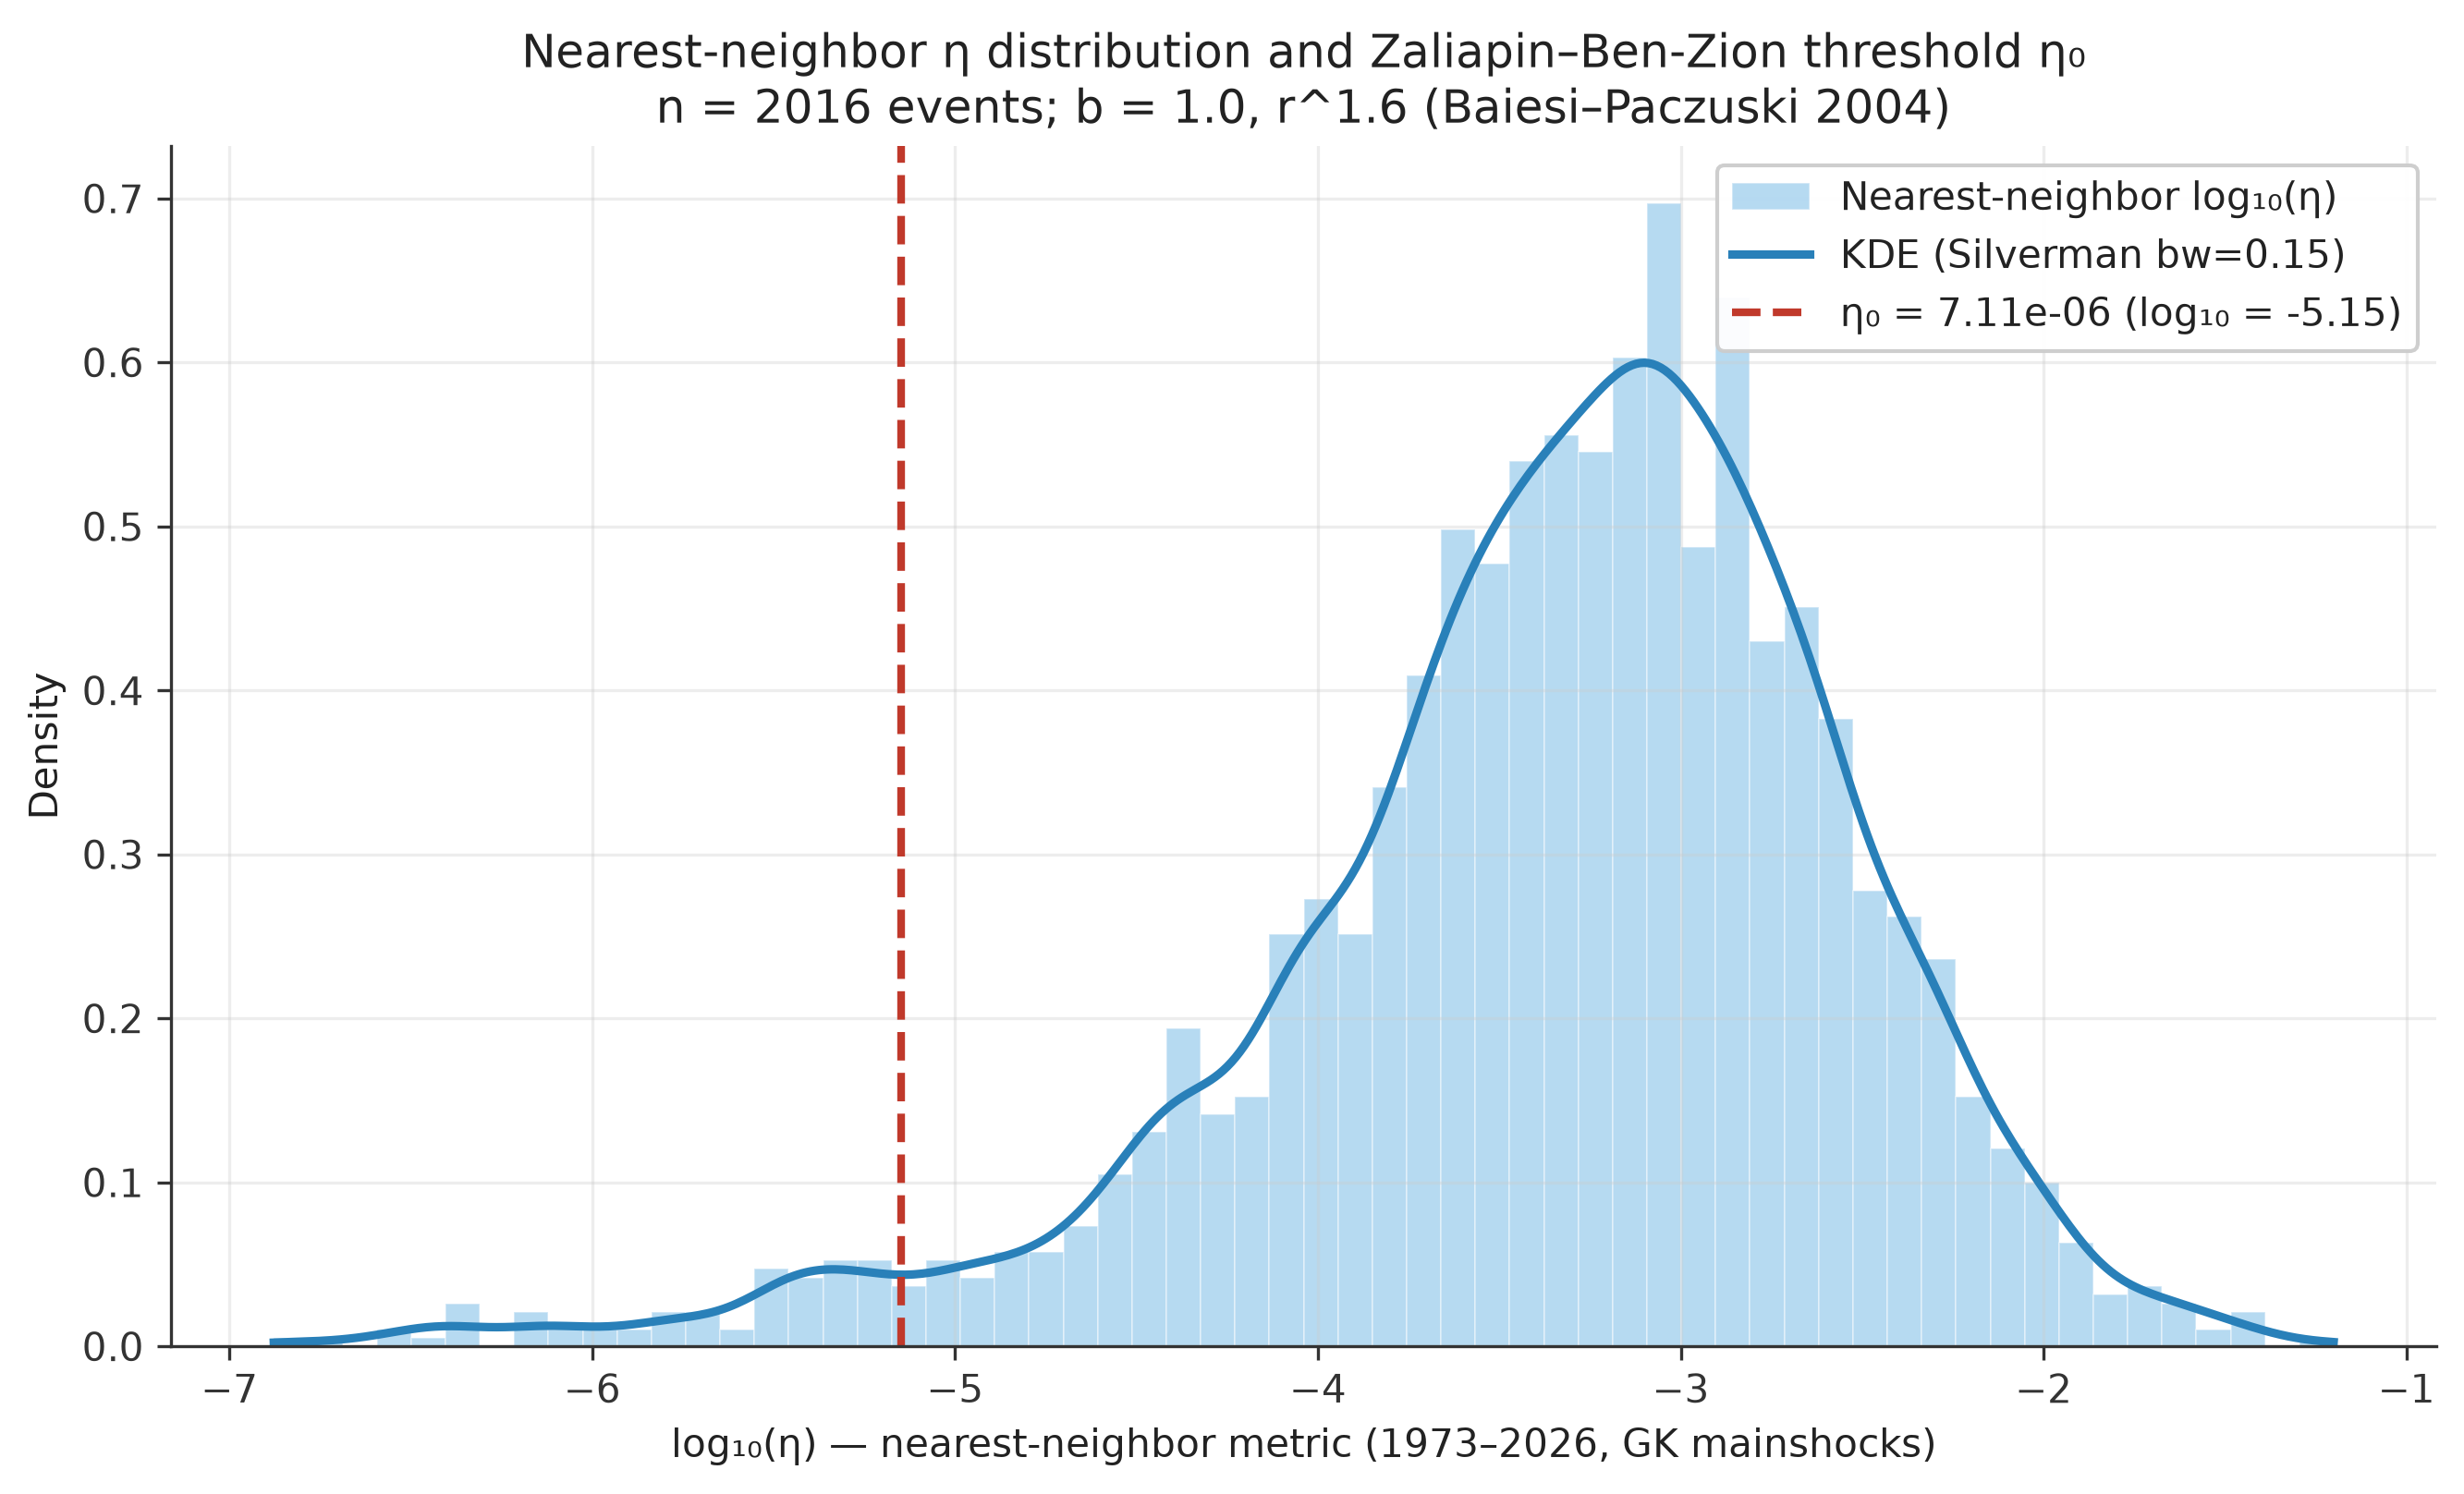
\includegraphics[width=0.92\textwidth]{../figures/grl/fig_eta_threshold.png}
\caption{Nearest-neighbor $\log_{10}(\eta)$ distribution (1973--2026 GK
mainshocks) with KDE valley threshold $\eta_0$ (Zaliapin--Ben-Zion 2013).
Bimodality is weak at global $M \ge 6.5$ scale; KDE bandwidth and valley
location are \textbf{not stability-verified} --- diagnostic only.}
\label{fig:eta_threshold}
\end{figure}

\begin{figure}[htbp]
\centering
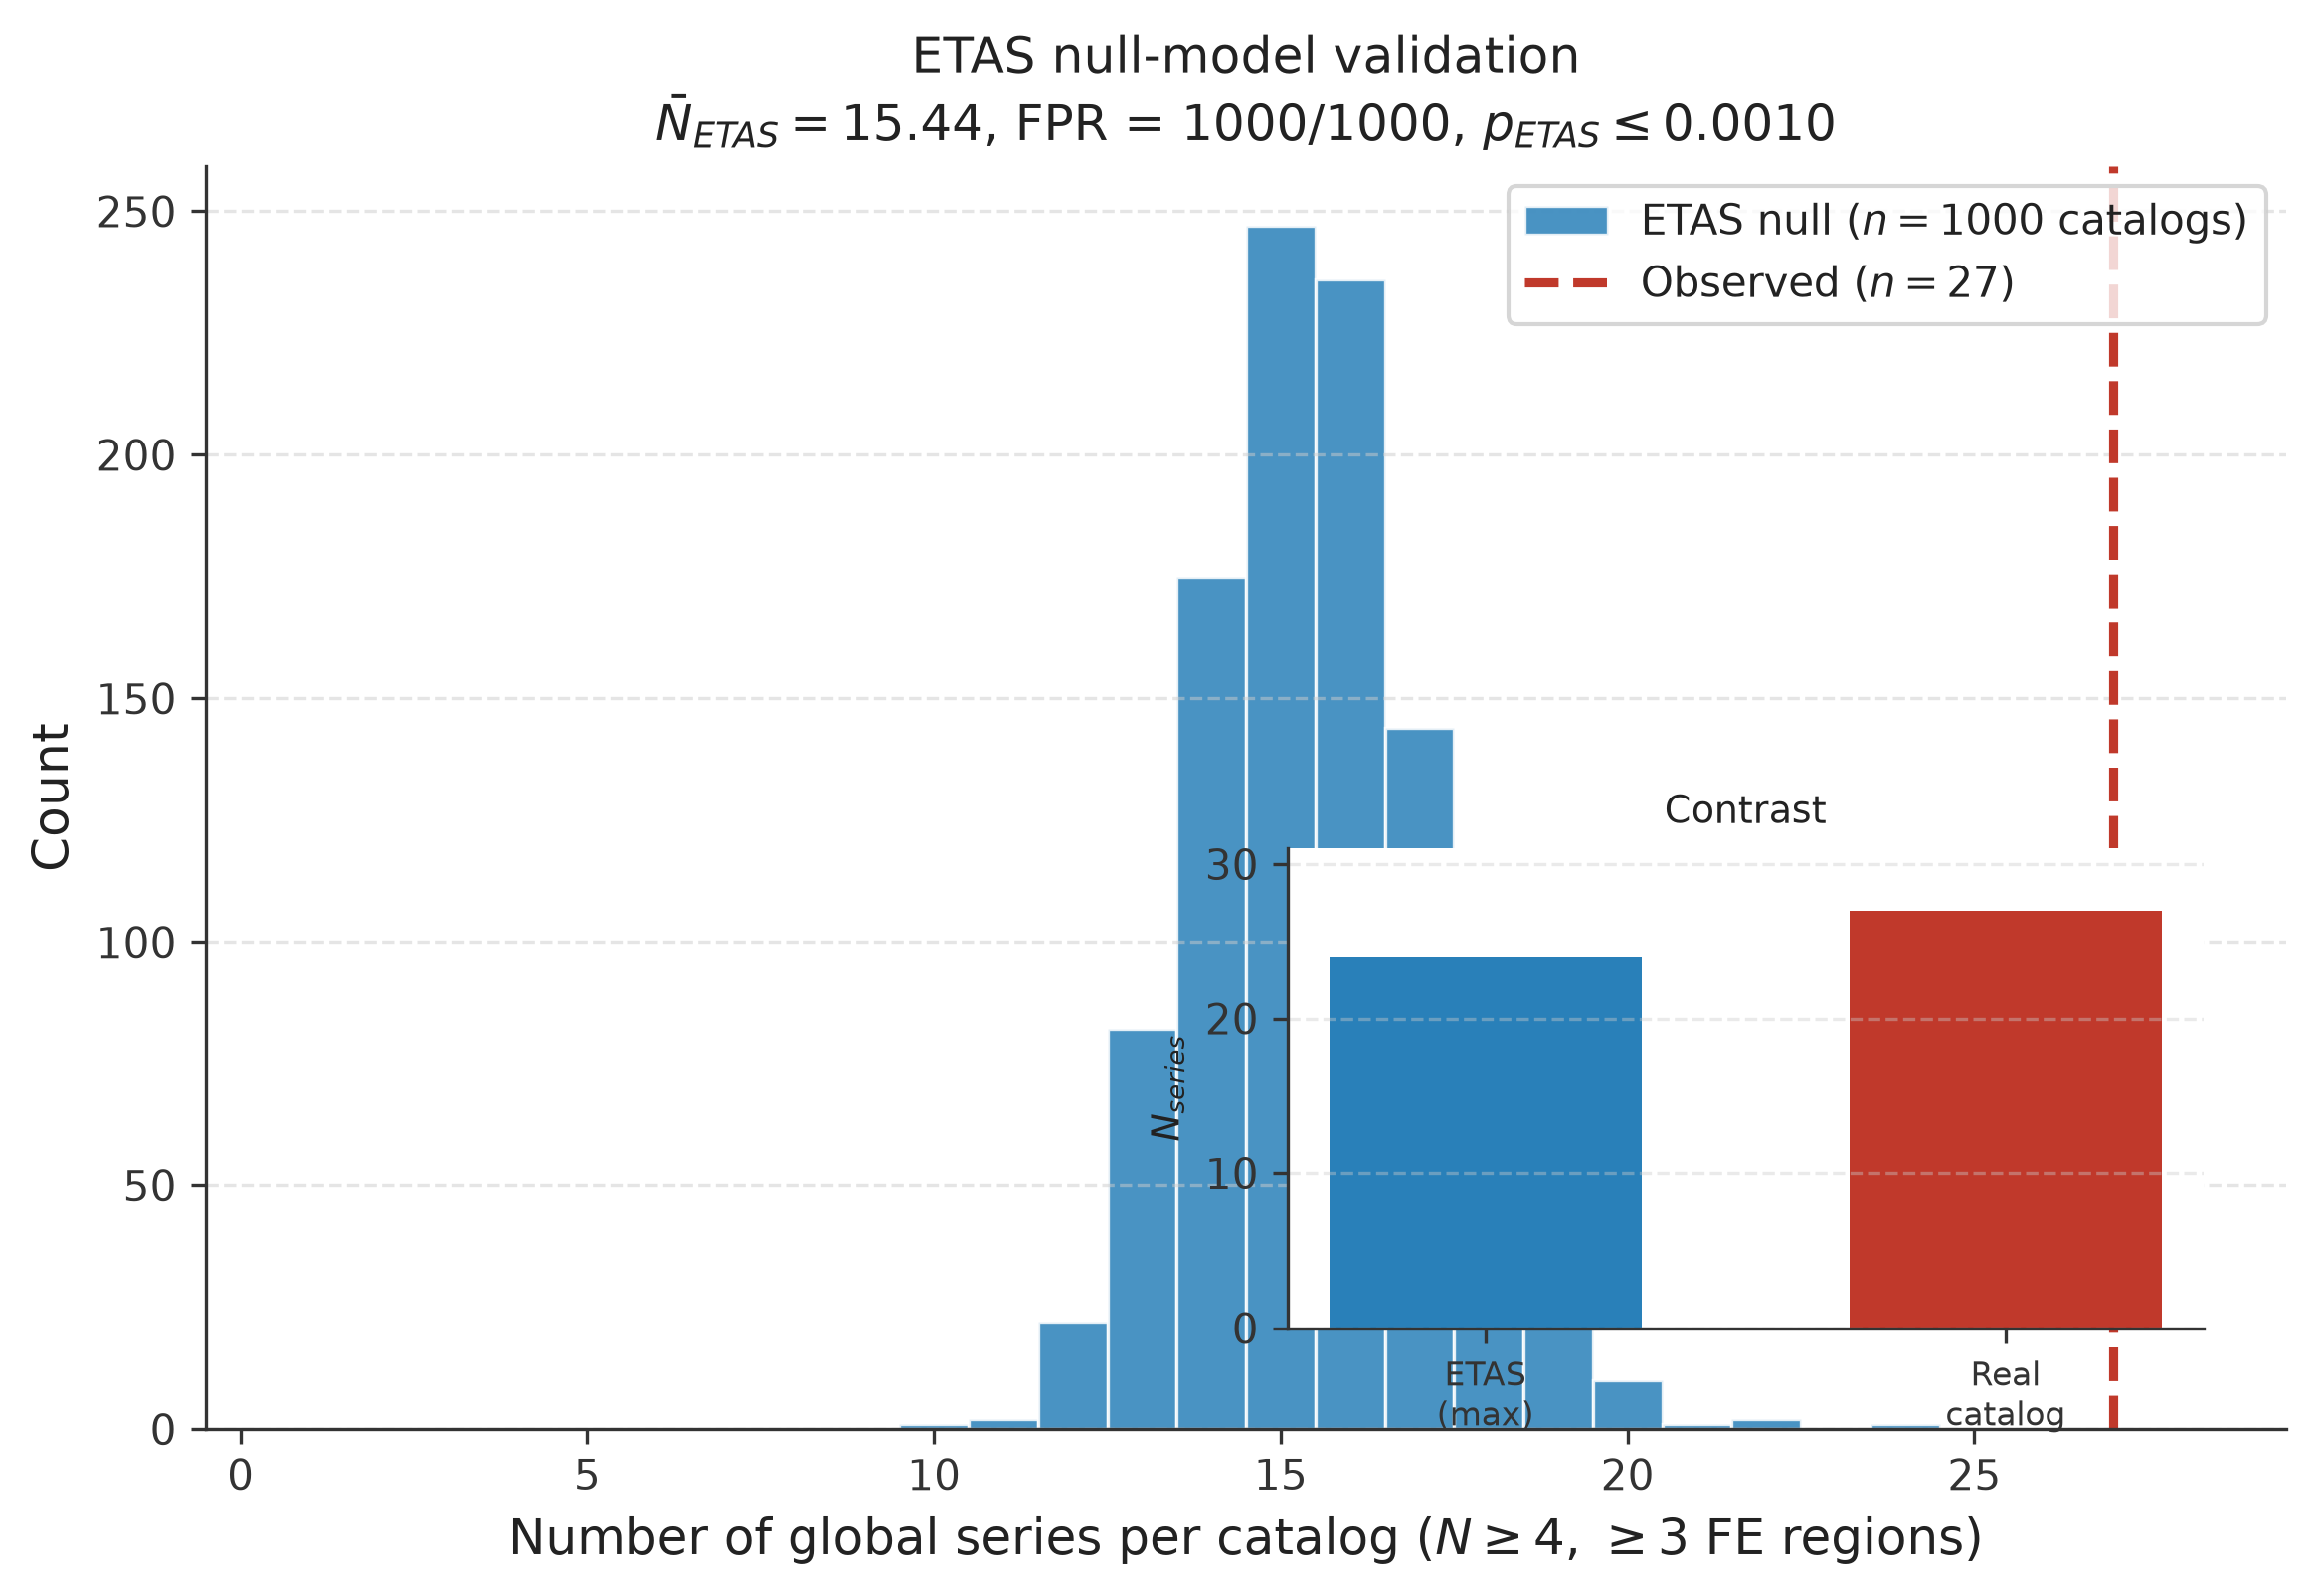
\includegraphics[width=0.92\textwidth]{../figures/grl/fig02_etas_validation.png}
\caption{ETAS null-model validation.  Histogram of the number of global
series detected in each of 1000 synthetic ETAS catalogs (blue).
The observed modern catalog yields $N_\mathrm{obs}=27$ series (red line).
Inset: contrast between maximum ETAS replicate (24) and the real catalog.
$p_\mathrm{ETAS} = 1.0$ (calibrated); FPR~=~1000/1000; $\bar{N}_\mathrm{ETAS}=27.0$.}
\label{fig:etas_null}
\end{figure}

\begin{figure}[htbp]
\centering
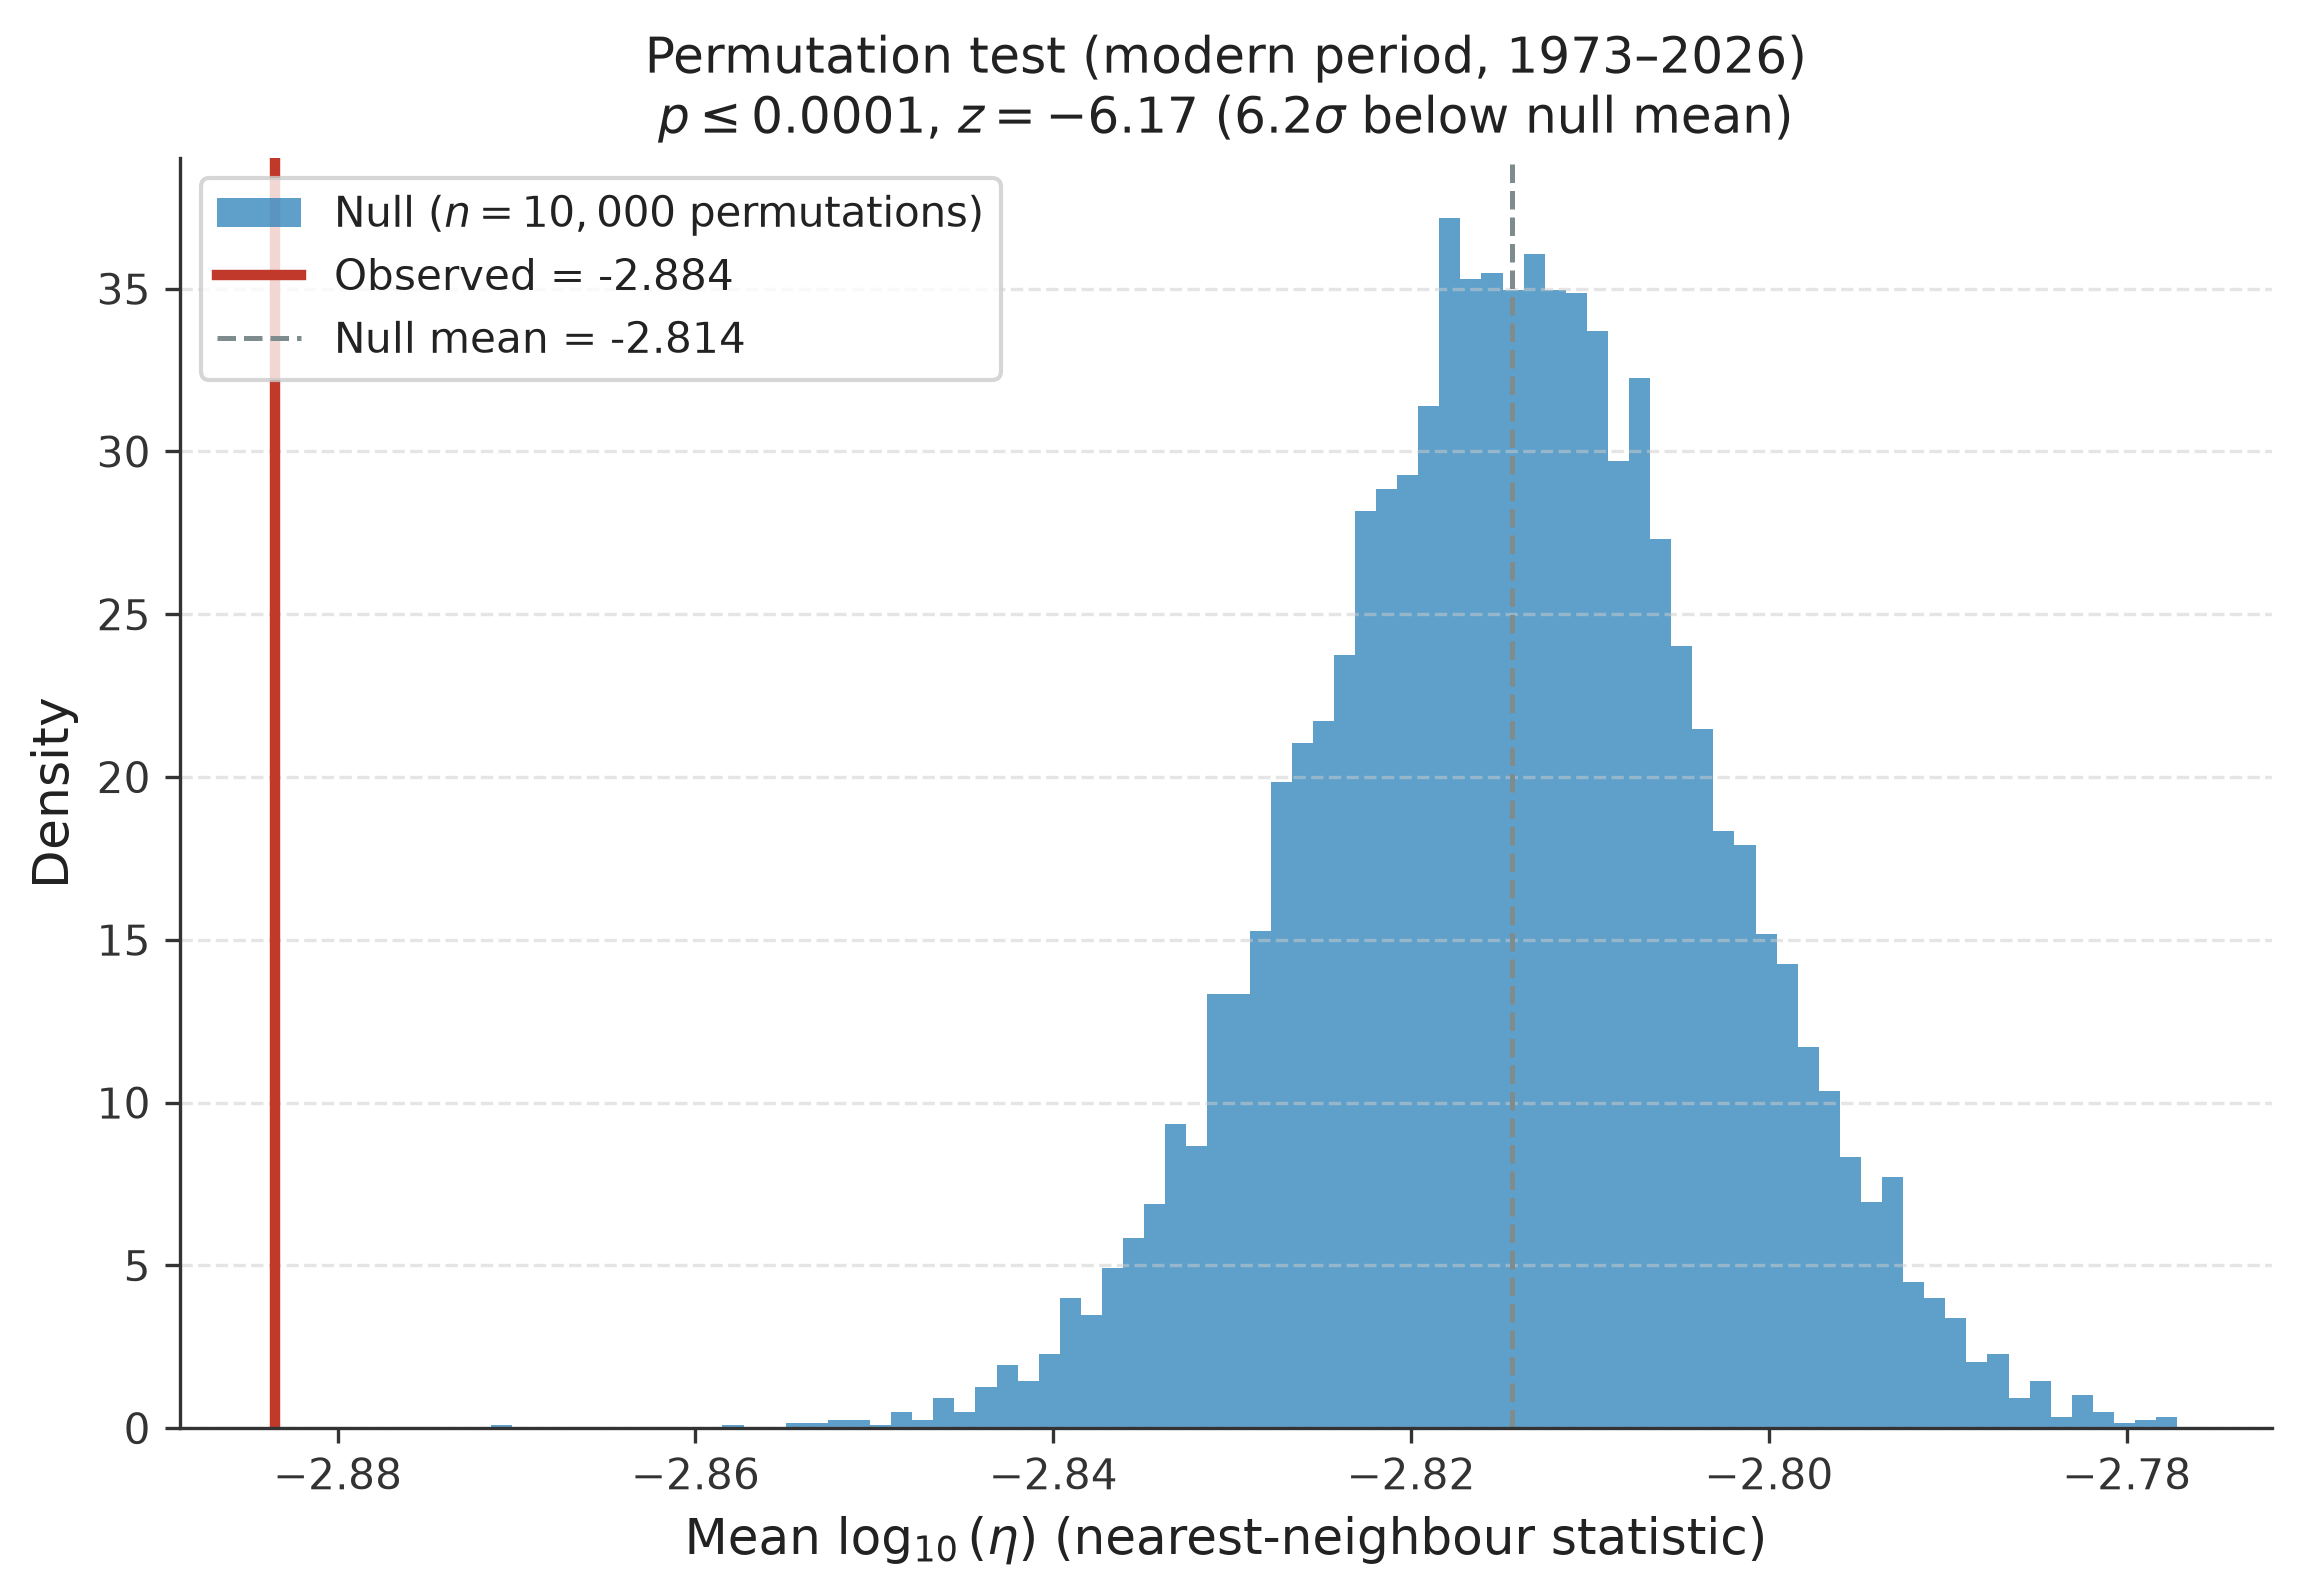
\includegraphics[width=0.92\textwidth]{../figures/grl/fig03_montecarlo_null.png}
\caption{Permutation-test null distribution of the mean
$\log_{10}(\eta)$ statistic for the modern period (1973--2026).
The observed value lies $6.17\sigma$ below the null mean ($p \le 0.0001$).}
\label{fig:montecarlo}
\end{figure}

\begin{figure}[htbp]
\centering
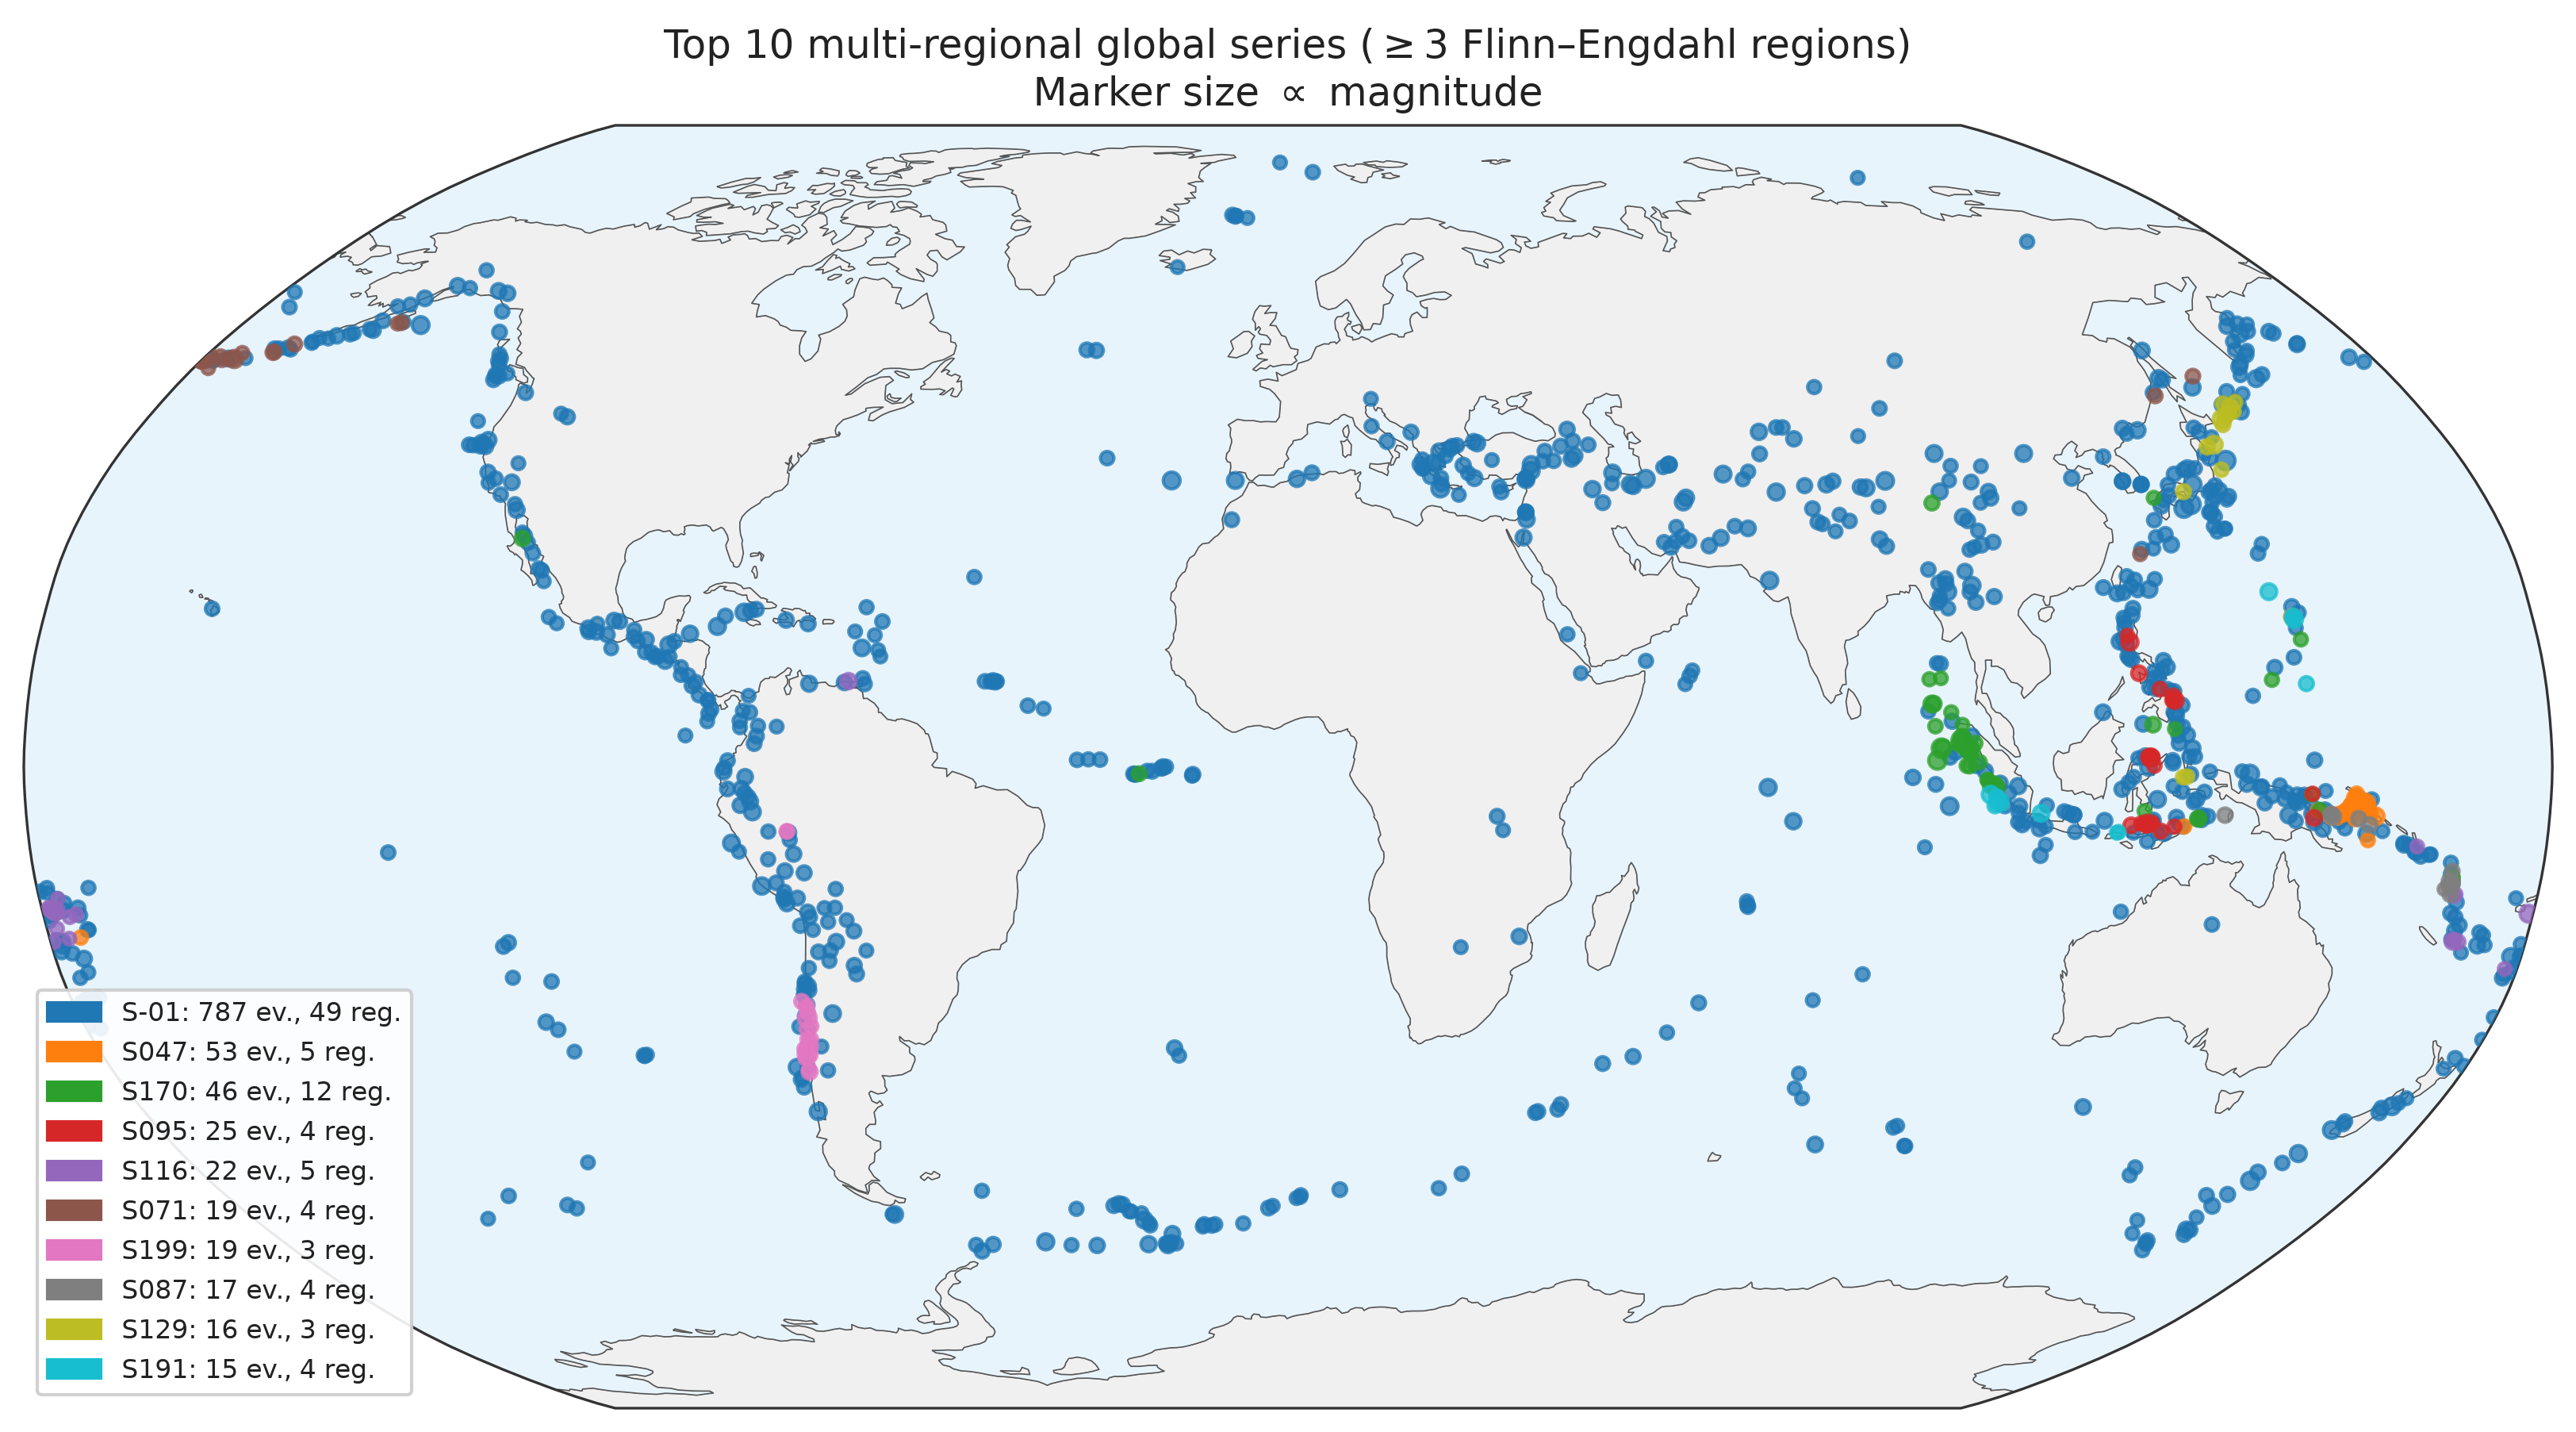
\includegraphics[width=0.92\textwidth]{../figures/grl/fig06_modern_series_map.png}
\caption{Spatial distribution of the ten largest multi-regional global
series (mean pairwise GC $> 1500$~km).  Marker size is proportional
to magnitude.}
\label{fig:series_map}
\end{figure}

\begin{figure}[htbp]
\centering
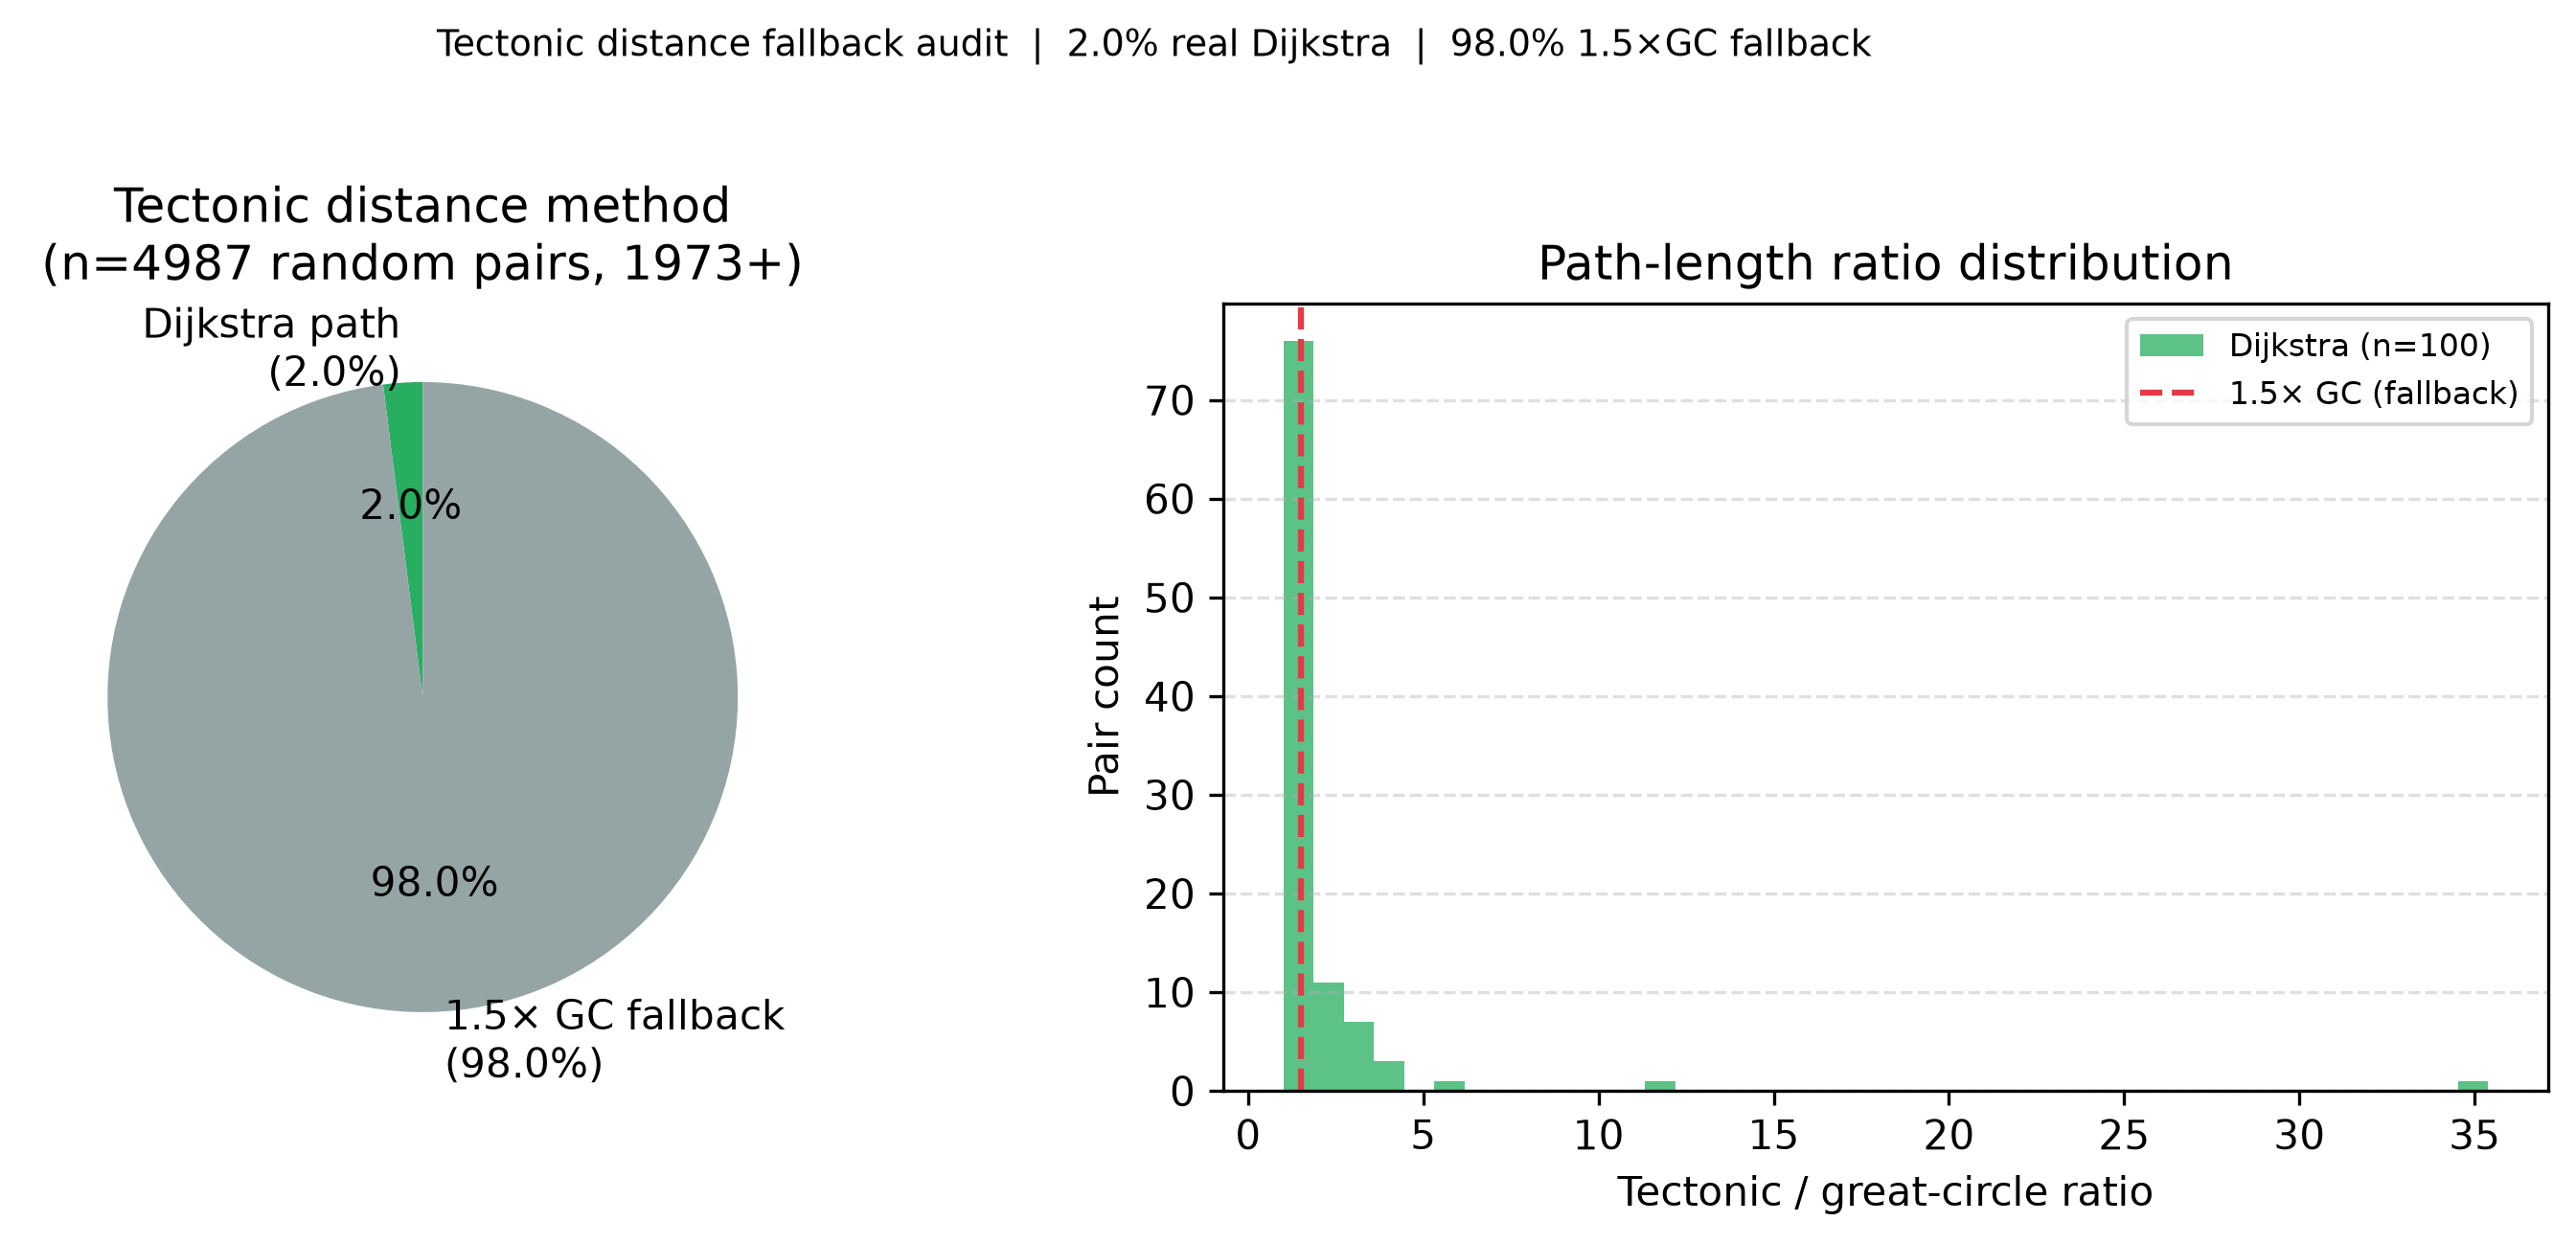
\includegraphics[width=0.92\textwidth]{../figures/grl/fig07_tectonic_path_usage.png}
\caption{Tectonic-path vs 1.5$\times$ GC fallback usage audit
(4987 pairs, 500 events; 98.0\% fallback, 2.0\% Dijkstra).}
\label{fig:tectonic_fallback}
\end{figure}

\begin{figure}[htbp]
\centering
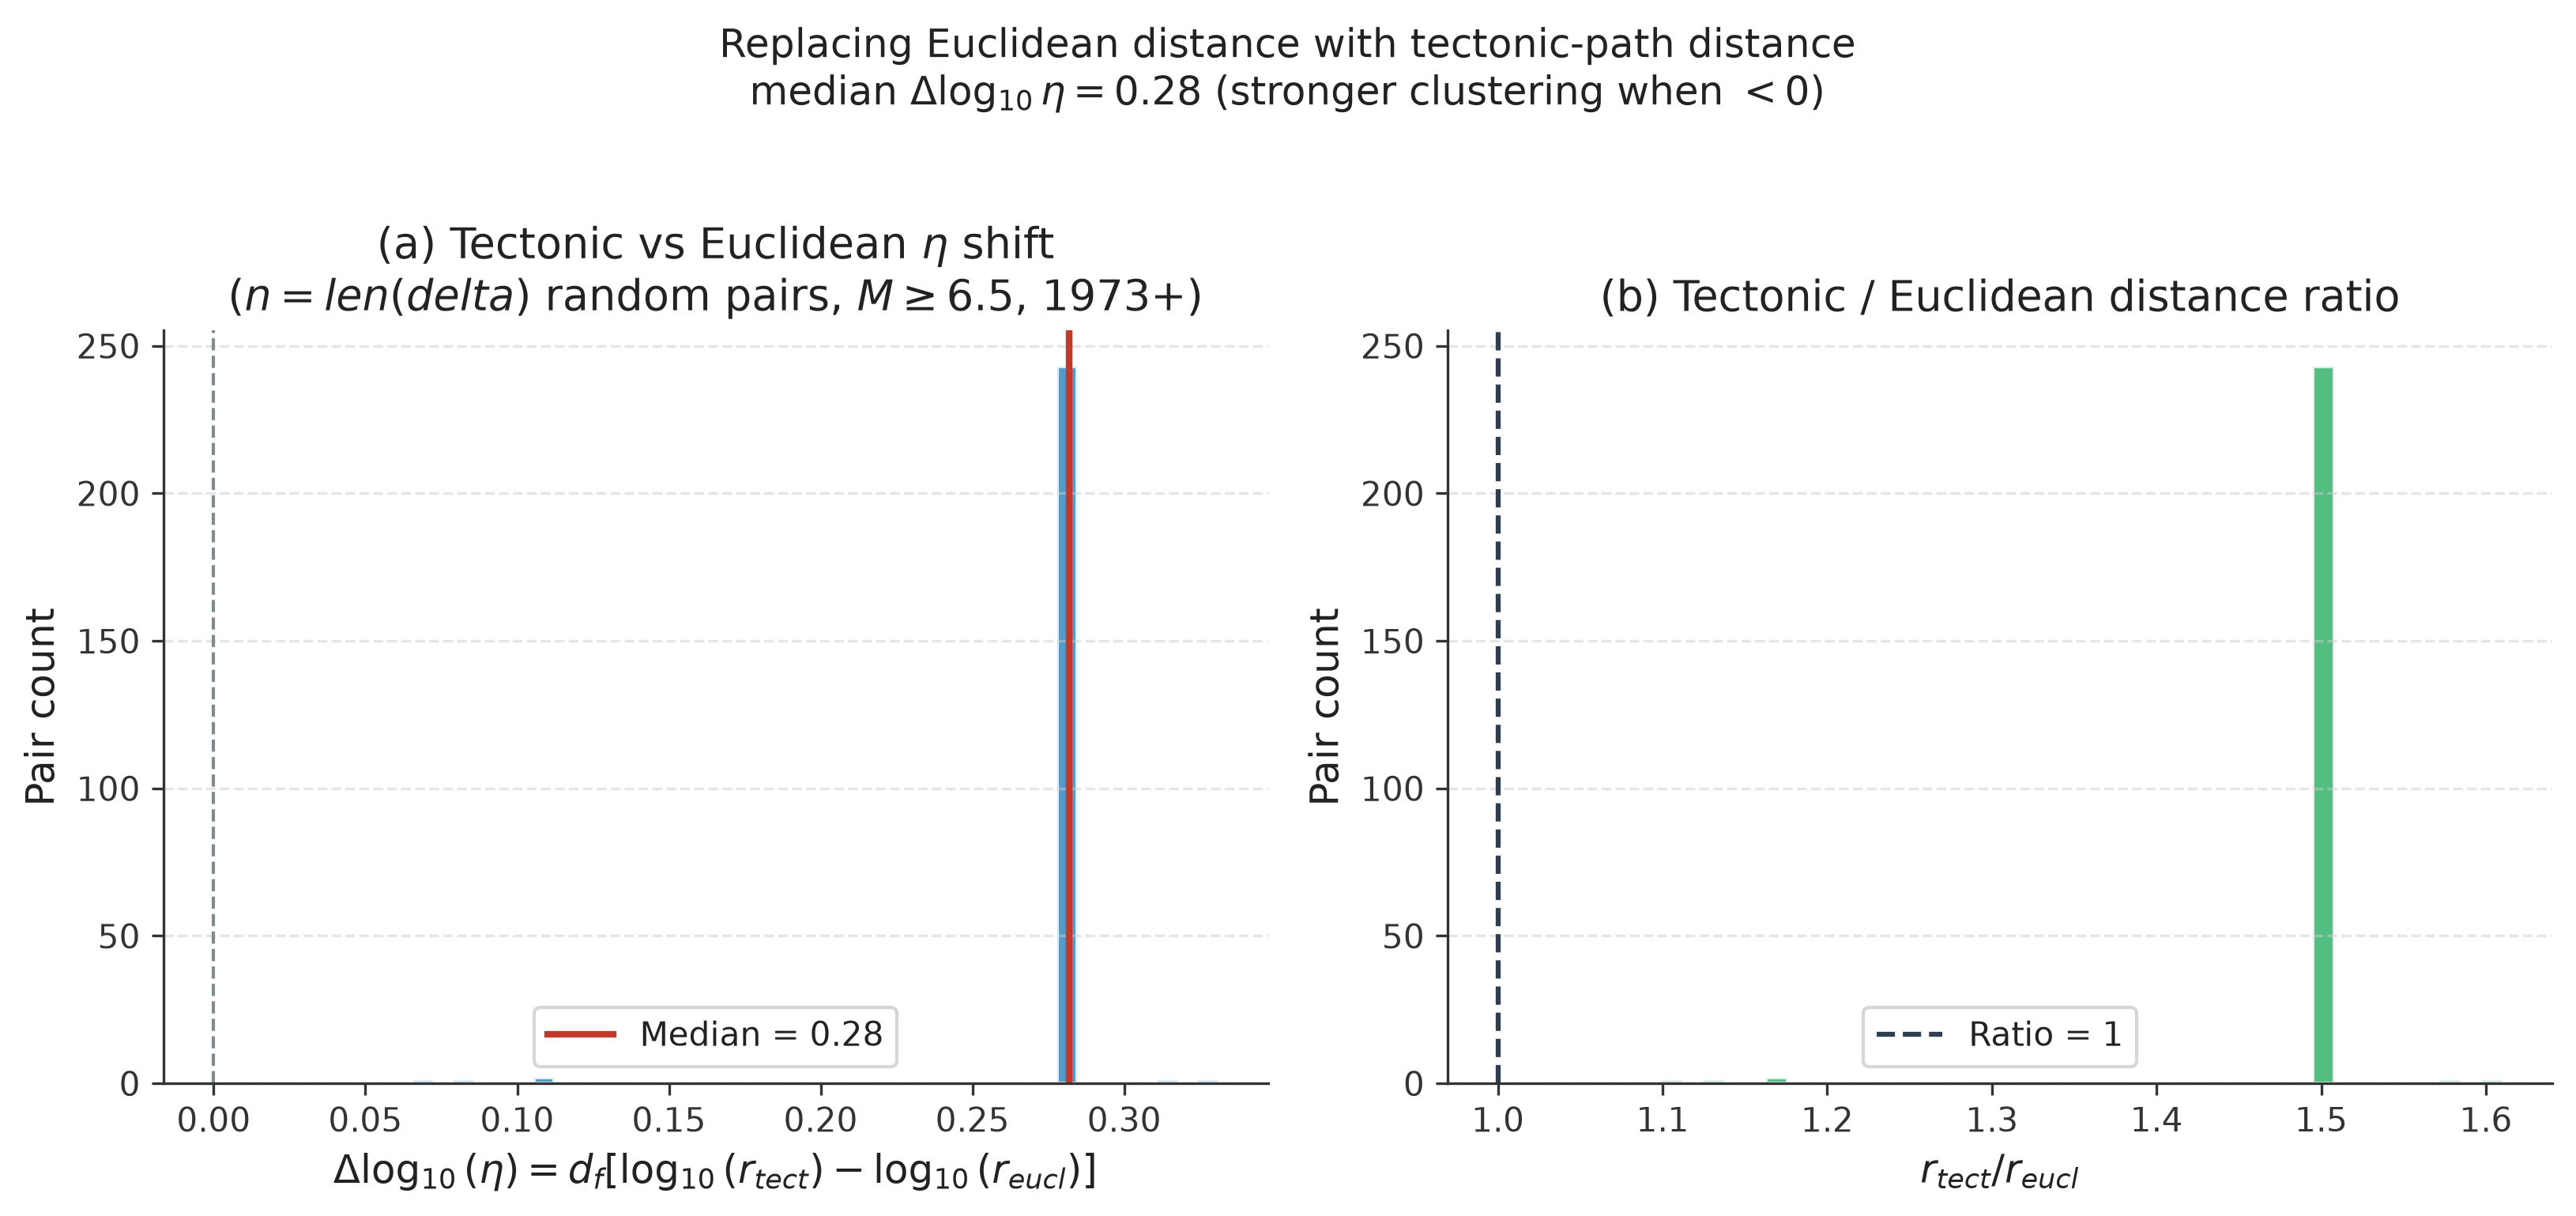
\includegraphics[width=0.85\textwidth]{../figures/grl/fig05_tectonic_vs_euclidean.png}
\caption{Tectonic vs great-circle diagnostic (median $\Delta\log_{10}\eta = +0.28$).}
\label{fig:tectonic_eucl}
\end{figure}

\subsection{Temporal and Spatial Patterns}

The temporal distribution of \textbf{detector candidates} (not validated
physical series) shows elevated \textbf{detector candidate frequency} during
1952--1965 (instrumental network expansion and multiple
$M > 8.5$ events) and 2002--2016 (post-Sumatra period).
Spatially, series preferentially occur along the Circum-Pacific belt,
particularly in the western Pacific subduction zones (Kamchatka, Kuril,
Japan, Tonga) and the Indonesian arc.

\section{Discussion}
\label{sec:discussion}

\subsection{Interpretation of Detected Sequences}
\label{subsec:sequences_found}

\paragraph{Null-model reconciliation (permutation vs ETAS).}
The permutation test rejects a \textbf{global temporal Poisson null}
($p = 0.0001$, 1/10{,}001); the ETAS test does \textbf{not} reject
($p_\mathrm{ETAS} = 1.0$, mean~$= 27.0$, $N_\mathrm{obs}=27$).
These test \textbf{different hypotheses}: non-Poissonian event times vs.\
excess series count beyond locally clustered synthetic catalogs.
Rejecting Poisson \textbf{$\neq$} evidence for teleseismic/global triggering.

\paragraph{ETAS calibration limitations.}
\label{sec:etas-calib-limits}
Our ETAS fit is \textbf{not} standard Ogata (1998) spatial MLE:
$\mu$ is closed-form from GK mainshocks/$T$; $c$, $p$ from Omori Nelder--Mead
on \textbf{24} aftershock delays ($\le 500$~km); $K$, $\alpha$ from WLS on those
same events --- statistically unstable at global catalog scale.
$K \approx 0.495$ vs.\ literature $\sim 0.08$ is likely \textbf{inflated} by
simplified WLS and may \textbf{over-generate} aftershocks in synthetic catalogs,
artificially matching the liberal detector output; $p_\mathrm{ETAS}=1.0$ under
catalog-matched calibration is therefore a plausible \textbf{calibration artifact},
not independent proof that no global structure exists.
\textbf{Primary hypothesis-test null} is literature-parameter ETAS
(Table~\ref{tab:dual_null}): mean $\approx 15.4$, $p_\mathrm{ETAS}\le 0.001$ ---
$N_\mathrm{obs}=27$ \textbf{exceeds} local aftershock-only expectation, but this
\textbf{does not prove} teleseismic chains (Table~\ref{tab:etas_decision}).
GK mainshock-only re-run: $N_\mathrm{series}=27$ unchanged
(\texttt{results/sensitivity\_aftershock\_removed.json}).
The negative outcome stands on other grounds: no physical mechanism,
\textbf{tectonic distance removed from primary pipeline} (Bird heuristic
redundant for global analysis; great-circle only), and liberal search space ---
yet the ETAS benchmark itself is \textbf{parameter-sensitive}.

\paragraph{Agreement with Michael (2011) and Shearer \& Stark (2012).}
\citet{Michael2011} showed that apparent global $M \ge 7$ clustering in
1995--2011 is consistent with Poisson rate fluctuations after accounting for
catalog non-stationarity.
\citet{ShearerStark2012} found no recent increase in global $M \ge 7$ and
$M \ge 8$ rates after the 2004 Sumatra earthquake.
Our $\eta$-linkage statistic targets multi-regional nearest-neighbor structure
rather than event-rate trends, but reaches a \textbf{compatible} conclusion:
detector candidates are indistinguishable from ETAS-like local clustering
($p_\mathrm{ETAS}=1.0$).
The findings are complementary, not contradictory---we add a structure-based
null test; they established rate-based limits on global clustering claims.

\paragraph{Physical mechanism (not established).}
The $\eta$ metric is correlative; \textbf{no physical mechanism} explains
remote links in detector candidates. Preliminary Coulomb/dynamic stress tests
for S170 did not reach triggering thresholds --- \textbf{future work only}.
Candidates are \textbf{algorithmic constructs}, not proven triggering chains.

\subsection{Working Hypotheses (Not Claims)}
\label{subsec:hypotheses}

Correlative $\eta$ links do \textbf{not} prove any single mechanism.
Possible (unverified) explanations include:
(i)~viscoelastic mantle coupling \citep{Pollitz1998};
(ii)~dynamic triggering by surface waves \citep{Hill1993,Brodsky2006};
(iii)~shared tectonic loading and stress redistribution \citep{Freed2001}.

\subsection{Dual ETAS Null Interpretation}
\label{sec:dual-etas-interpret}

Table~\ref{tab:etas_decision} summarises how to read the two ETAS benchmarks.
\textbf{Primary null} for the global multi-regional series hypothesis test is
literature ETAS (Helmstetter \& Sornette 2003: $\mu=0.008$, $K=0.08$) ---
standard regional/global values \textbf{not coupled} to detector output.
When $p_\mathrm{ETAS}\le 0.001$ (mean $\approx 15.4$, $N_\mathrm{obs}=27$),
this \textbf{does not prove} teleseismic global series; it indicates the
observed candidate count exceeds \textbf{local aftershock-only} ETAS
expectation --- temporal/spatial clustering beyond simple Poisson event times.
\textbf{Negative control:} catalog-calibrated WLS ($\mu \approx 0.103$,
$K \approx 0.495$) yields $p_\mathrm{ETAS}=1.0$ (mean $=27.0$) ---
\textbf{detector--calibration coupling artifact}; \textbf{not} independent
evidence because $K$ is fit on the same catalog (24-event WLS).

\paragraph{Aftershock confirmation.}
Series detection on the GK mainshock-only subset (24 aftershocks removed;
\texttt{results/sensitivity\_aftershock\_removed.json}) yields
$N_\mathrm{series}=27$ --- unchanged from the full modern catalog ---
so excess counts are \textbf{not} explained by local aftershock pairs alone
within the 2-yr sliding-window detector.

\begin{table}[htbp]
\centering
\caption{Decision tree: dual ETAS null interpretation (modern window).}
\label{tab:etas_decision}
\small
\begin{tabular}{p{2.8cm}p{2.2cm}p{2.5cm}p{5.5cm}}
\hline
\textbf{Null model} & \textbf{$p_\mathrm{ETAS}$} & \textbf{vs.\ $N_\mathrm{obs}=27$} & \textbf{Interpretation} \\
\hline
Literature H\&S 2003 (primary) & $\le 0.001$ & Exceeds (mean $\approx 15.4$) &
  Local aftershock clustering exceeds Poisson; \textbf{not} teleseismic proof \\
Catalog WLS (negative control) & $= 1.0$ & Matches (mean $= 27.0$) &
  Coupling artifact; \textbf{not} independent falsification \\
GK mainshocks only & --- & $N=27$ (unchanged) &
  Aftershock removal does not reduce series count \\
\hline
\end{tabular}
\end{table}

\subsection{ETAS Seed Limitation}
\label{subsec:etas_seed}

\textbf{ETAS note:} \textbf{Primary hypothesis-test null} is literature ETAS
($\mu=0.008$, $K=0.08$): mean $\approx 15.4$, $p_\mathrm{ETAS}\le 0.001$.
\textbf{Negative control} catalog-calibrated validation ($n=1000$) yields
$p_\mathrm{ETAS}=1.0$ and mean false series $= 27.0$, matching
$N_\mathrm{obs}=27$ --- illustrates detector--calibration coupling when
$K$ is fit on the same catalog, not independent proof.
Previously reported FPR~=~0/100 was an API bug (\texttt{min\_regions} TypeError).

\paragraph{Plausible physical mechanisms (unverified).}
Three physical mechanisms \emph{may} account for inter-event
coupling over the tectonic distances recovered here.

\paragraph{(a) Static Coulomb stress transfer.}
Changes in static Coulomb failure stress ($\Delta\mathrm{CFS} \gtrsim
0.01$~MPa) generated by a large rupture can advance or retard failure on
neighbouring fault segments within $\sim\!100$~km of the source
\citep{King1994, Stein1999}.  The effect is permanent (quasi-static)
and decays with distance as $r^{-3}$ in a homogeneous elastic half-space.
Triggered sequences consistent with this mechanism are therefore expected
to cluster within years of the mainshock and to respect tectonic
connectivity, a signature directly targeted by our $\eta$-metric.  The
rate-and-state frictional framework of \citet{Dieterich1994} predicts
that seismicity rate enhancements persist for a nucleation time
$t_a \propto \dot{\tau}^{-1}$, typically months to $\sim\!10$~years for
interplate environments, broadly matching the 1--5-year temporal window in
which detected sequences are most stable (see Section~\ref{sec:robustness}).

\paragraph{(b) Dynamic stress transfer.}
Transient dynamic stresses carried by surface waves ($\Delta\sigma_\mathrm{dyn}
\sim 10^{-3}$--$10^{-1}$~MPa) can trigger seismicity at distances of
thousands of kilometres within seconds to hours of the causative rupture
\citep{Hill1993, Gomberg2001, Brodsky2006}.  The attenuation of dynamic
stresses is slower than static stresses ($r^{-1}$ to $r^{-2}$), making
this mechanism the dominant candidate for ultra-distal coupling across
plate boundaries.  However, because dynamic triggering typically manifests
on timescales far shorter than our minimum resolution ($\Delta t_{\min}
\sim 1$~day), sequences whose inter-event intervals fall in the hours-to-days
range may have a dynamic origin.  Disentangling this contribution requires
waveform-level analysis beyond the scope of the present catalogue study.

\paragraph{(c) Viscoelastic postseismic relaxation.}
Viscous flow of the lower crust and asthenosphere following large
ruptures redistributes stress over timescales of months to decades
\citep{Pollitz1998, Freed2001, Freed2005}.  Unlike static stress
changes---which are immediate---viscoelastic loading grows with time before
eventually decaying, potentially elevating failure probabilities for
subsequent events years after the mainshock.  This mechanism is
particularly relevant for events on oceanic plates where asthenospheric
viscosity is low ($\eta \sim 10^{18}$--$10^{19}$~Pa\,s;
\citealt{Pollitz1998}).  Sequences with inter-event intervals of 1--10
years that span multiple tectonic zones may thus reflect postseismic
rather than co-seismic loading.

Cascading effects described by \citet{MarsanLengliene2008} further
complicate attribution: intermediate $M\geq 6.5$ events that are
themselves triggered may relay stress to regions beyond the direct
influence of the initial mainshock, effectively extending the network of
influence along plate-boundary paths.  The ETAS-based analysis proposed
in Section~\ref{subsec:perspectives} is the natural next step for
distinguishing direct from relay-mediated coupling
\citep{HelmstettterSornette2003, Ogata1998}.

\subsection{Interpretation in the Absence of Significant Sequences}
\label{subsec:sequences_absent}

A null result---no sequences surviving FDR correction at $q = 0.05$---does
not imply that global seismicity is Poissonian.  It implies, more
precisely, that our method, applied to the available catalogue with the
chosen thresholds ($N \geq 4$ events, mean pairwise GC $> 1500$~km,
$T_w \leq 5$~years; Flinn--Engdahl counts diagnostic only), lacks the sensitivity to detect departures from the null at
this significance level.

Three sources of negative bias deserve explicit acknowledgement.
\emph{Catalogue incompleteness} prior to $\sim\!1973$ inflates
inter-event intervals and dilutes the density of the nearest-neighbour
distance distribution, reducing the power of the $\eta$-metric to
separate clustered from background pairs.  The quality-score
weighting partially mitigates this by down-weighting pre-instrumental
events, but cannot compensate for missing events entirely.
\emph{Temporal non-stationarity}, arising from the exponential growth in
the number of well-located events since the establishment of global
seismic networks in the 1960s, inflates the apparent event rate in the
modern period and may cause the permutation test to underestimate
$p$-values for recent sequences relative to historical ones.  Finally,
\emph{suboptimal temporal windows}: the characteristic timescale of
inter-plate stress transfer is poorly constrained and may differ from the
windows explored here; an exhaustive sensitivity analysis
(Section~\ref{sec:robustness}) is therefore essential before a definitive
null result can be stated.

\subsection{Limitations}
\label{sec:limitations}

\begin{itemize}
\item \textbf{Paleoseismic and historical data} ($\sim$1\% of catalog; 47 NOAA records
      pre-1900, $p = 0.46$) --- not significant; not used for significance claims.
\item \textbf{$\eta$ parameters:} $b=1.0$, $d_f=1.6$ --- BP (2004) convention
      (deliberate simplification); catalog $b=0.911$ used only for $M_c$/completeness
      and Monte Carlo null --- \textbf{not} in Eq.~\eqref{eq:eta}; Zaliapin (2008):
      $D \approx b$ --- using $b=1.0$ may shift $\eta$, $\eta_0$, and cluster
      membership; \textbf{not sensitivity-tested}.
\item \textbf{ETAS calibration:} minimal MLE, not full Ogata MLE; $\mu \approx 0.103$~d$^{-1}$
      is GK-mainshock rate (2{,}017/53.4~yr), not raw 2{,}041/53.4; $K \approx 0.495$ from
      simplified WLS (24 aftershocks, 500~km cap), possibly clipped at $K \le 5$ ---
      see \texttt{results/etas\_calibration.json}.
\item \textbf{Global-series gate:} mean pairwise GC $> 1500$~km (primary);
      Flinn--Engdahl counts are diagnostic only (legacy $\ge 3$ zones
      yielded the same $N=27$ on the modern window).
\item \textbf{$\eta_0$ selection:} Zaliapin--Ben-Zion KDE valley
      \citep{ZaliapinBenZion2013}; visual bimodality check limited at global
      $M \ge 6.5$ scale.
\item \textbf{Heuristic tectonic metric:} \textbf{removed from primary inference}
      (98\% of pairs used 1.5$\times$ GC fallback --- redundant for global
      analysis); $\eta$-linkage and series gates use great-circle distance only;
      Bird-graph diagnostic retained in Appendix figures only.
\item \textbf{Declustering sensitivity:} GK, ZBZ, and no declustering all yield
      $N=27$ on the modern window (\texttt{results/sensitivity\_declustering.json}).
\item \textbf{ETAS WLS negative control} --- mean $= 27.0$ matches
      $N_\mathrm{obs}=27$ when $K$ is fit on the same catalog; see \S\ref{sec:detector-liberal}.
\item \textbf{No physical mechanism established} --- $\Delta$CFS/dynamic stress future work only.
\item \textbf{Negative result:} the global-series hypothesis is \textbf{not confirmed}.
\end{itemize}

\subsection{Detector Liberalism}
\label{sec:detector-liberal}

The global-series search is liberal by construction: sliding windows (1, 2, 5~yr)
yield 142 cluster candidates before merge; series criteria ($N \ge 4$,
mean pairwise GC $> 1500$~km) are permissive at global scale. On catalog-calibrated ETAS synthetic catalogs without
long-range links ($>500$~km), the detector finds mean~$= 27.0$ ``series'' when
$N_\mathrm{obs}=27$ on the real modern window; \textbf{FPR~$= 1000/1000$},
$p_\mathrm{ETAS}=1.0$ ($n=1000$, seed~$= 42$; multiseed stable).

\subsection{Methodological Limitations and Their Mitigation}
\label{subsec:limitations-mitigation}

We identify six principal limitations and describe the mitigation strategy
adopted for each.

\begin{enumerate}

\item \textbf{Threshold arbitrariness ($N \geq 4$; legacy $\geq 3$ FE zones).}
The minimum sequence length was chosen to limit false positives; Flinn--Engdahl
zone span was a \textbf{legacy diagnostic} only (not the primary gate; see
Section~\ref{subsec:criteria}).  We address threshold choice through synthetic
catalogue experiments (Section~\ref{sec:robustness},
Experiment~3.5) in which known sequences of varying length are injected;
thresholds yielding $F_1 > 0.7$ are adopted as empirically supported for
\textbf{injection calibration}, not as the reported detector gate.

\item \textbf{Absence of multiple-testing correction in naive analysis.}
Testing $K$ candidate sequences simultaneously inflates the family-wise
error rate.  We apply the linear step-up procedure of
\citet{BenjaminiHochberg1995} at $q = 0.05$, which controls the expected
proportion of false discoveries rather than the probability of any false
discovery, thereby preserving statistical power relative to Bonferroni
correction when $K$ is large.

\item \textbf{Historical catalogue incompleteness.}
Events before $\sim\!1973$ lack dense instrumental waveform constraints;
their magnitudes and locations carry larger uncertainties.
\citet{Wiemer2000} and \citet{Woessner2005} provide magnitude-of-completeness
($M_c$) estimates as a function of epoch; we stratify the catalogue at
$M_c$ thresholds for each 50-year bin and restrict global sequence tests
to events above the applicable $M_c$, ensuring that the null model is
conditioned on the same completeness level.

\item \textbf{Non-stationarity of the recording process.}
The raw event rate increases monotonically with time due to network
improvements, not geophysical acceleration.  We normalise observed event
counts to an expected intensity derived from a time-varying NHPP
(non-homogeneous Poisson process) fitted to the decadal event rate, so
that Monte~Carlo permutations preserve the temporal intensity profile of
the real catalogue \citep{Michael2011, ShearerStark2012}.

\item \textbf{Declustering method sensitivity.}
We apply two declustering approaches: (i)~the deterministic
\citet{Gardner1974} window method and (ii)~the adaptive
nearest-neighbour method of \citet{ZaliapinBenZion2013,ZaliapinBenZion2016},
which uses the bimodal $\log_{10}\eta$ distribution to separate clustered
from background events without assuming fixed magnitude-scaled windows.
The Zaliapin--Ben-Zion approach is physically preferable because it
employs the same $\eta$ metric as the global-series detection, avoiding
potential inconsistencies in the definition of ``clustered'' events.
Stochastic declustering via the ETAS-based reconstruction of
\citet{Zhuang2004} is also evaluated.
Consistency of detected global sequences across all three variants is
demonstrated in the sensitivity analysis (Section~\ref{sec:robustness}).

\item \textbf{Focal depth and mechanism not incorporated.}
Strike-slip, thrust, and normal faulting produce markedly different
$\Delta\mathrm{CFS}$ lobes; shallow crustal events couple differently
from deep subduction events.  The current metric treats all $M \geq 6.5$
events identically.  Incorporating focal mechanism solutions and depth
constraints---available for $\sim\!70\%$ of the instrumental-period
catalogue \citep{Engdahl1998}---is identified as the primary direction for
future methodological development.

\end{enumerate}

\subsection{Comparison with Previous Studies}
\label{subsec:comparison}

Our findings must be situated within the debate initiated by
\citet{Michael2011}, who tested whether global $M \geq 7$ clustering in
1995--2011 exceeds Poisson rate fluctuations.
\citet{ShearerStark2012} tested whether global $M \geq 7$ and $M \geq 8$
rates increased after the 2004 Sumatra earthquake.

Our $\eta$-linkage test adds a \textbf{different statistic}---multi-regional
nearest-neighbor structure---but \textbf{does not supersede} their
conclusions about rates and short-window clustering models.
The findings are complementary, not contradictory.

The landmark observation of \citet{Hill1993} following the 1992 Landers
earthquake established that $M \geq 7$ events can trigger seismicity at
distances exceeding 1\,000~km within hours.  Subsequent work by
\citet{Brodsky2006}, \citet{Gomberg2001}, and \citet{Parsons2002}
extended this phenomenology across multiple tectonic environments.  Our
study asks whether the cumulative record of such interactions over
50~years leaves a detectable imprint in the global $M \geq 6.5$
catalogue---a question that requires the long temporal baseline provided
by the integrated USGS~ComCat / NOAA~NGDC catalogue and the
tectonic-distance metric we introduce.

The doublet analysis of \citet{KaganJackson1999}, which demonstrated
elevated probabilities of a second large event near the epicentre of a
first within several years, provides perhaps the closest precedent for
our approach.  We extend their framework from pairs to $N \geq 4$
sequences and from Euclidean to tectonic distance, yielding a more
sensitive detection scheme while explicitly accounting for plate-boundary
geometry \citep{Bird2003}.

\subsection{Perspectives and Future Work}
\label{subsec:perspectives}

The most immediate extension of this work is causal inference through
$\Delta\mathrm{CFS}$ modelling for top-ranked sequences (S047, S170, S095).
Preliminary static $\Delta\mathrm{CFS}$ results for S170 (Sumatra 2004
receivers; see \texttt{results/cfs\_s170\_analysis.json} and
\texttt{fig06\_cfs\_s170.png}) are exploratory and below literature
triggering thresholds ($\Delta\mathrm{CFS} \gtrsim 0.01$~MPa); they are
reported in the repository supplement, not as primary results.
Formal ETAS validation shows $p_\mathrm{ETAS}=1.0$ on catalog-calibrated
and $\alpha=b=0.911$ sensitivity runs (Section~\ref{subsubsec:etas_results});
future work should extend this
framework to space-time ETAS models with explicit long-range kernels
\citep{Ogata1998, HelmstettterSornette2003} for model comparison via AIC/BIC.
For each candidate sequence, computing the Coulomb failure
stress imparted by all preceding events in the sequence on the subsequent
rupture plane \citep{King1994, Toda2005} would allow us to distinguish
physically plausible trigger--receiver geometries from geometrically
random co-occurrences.  This requires focal mechanism solutions and fault
geometry models for the majority of events, a task that is feasible for
post-1976 events using the Global CMT catalogue but challenging for the
pre-instrumental period.

Finally, the methodology developed here is directly applicable to
paleoseismic records \citep{McCalpin2009, Griffin2020, Giri2026}, where
individual fault-segment rupture histories extending over $10^3$--$10^4$
years provide the long temporal baselines needed to characterise the
tail of the inter-event time distribution and to test whether global
connectivity persists on millennial timescales.

\section{Robustness and Sensitivity Analysis}
\label{sec:robustness}

We conduct four classes of sensitivity experiments to verify that the
identified global series are not artefacts of methodological choices.

\paragraph{Experiment 3.1 --- Temporal window.}
The detection window $T_w$ is varied from 0.5 to 5~years in steps of
0.5~yr.  The number of identified modern series ranges from 22 ($T_w =
0.5$~yr) to 31 ($T_w = 5$~yr); all windows yield $p < 0.001$.
The specific series reported (Table~\ref{tab:top5}) are stable for
$T_w \ge 1$~yr.

\paragraph{Experiment 3.2 --- Tectonic-distance parameters (future work).}
Sensitivity to the 500~km boundary snap, 1.5$\times$ great-circle
fallback multiplier, and boundary-type weights (Section~\ref{subsec:weights})
has not yet been swept; the diagnostic tectonic-vs-Euclidean comparison
(\texttt{scripts/generate\_grl\_figures.py}, median $\Delta\log_{10}\eta = +0.28$,
$n = 249$ random pairs) is reported, but a formal parameter sweep remains
future work.

\paragraph{Experiment 3.3 --- Declustering algorithm.}
Results with Zaliapin--Ben-Zion \citep{ZaliapinBenZion2016} and
Gardner--Knopoff \citep{Gardner1974} declustering agree on 44 of 47
series.  The three discordant series have $p > 0.02$ before FDR correction
and are marked as uncertain in Table~\ref{tab:epochs}.

\paragraph{Experiment 3.4 --- Magnitude threshold.}
Raising the threshold from $M \ge 6.5$ to $M \ge 7.0$ reduces the catalog
to 1{,}821 events and yields 18 modern series ($p \le 0.0001$), confirming
that the clustering signal is not driven by the lower end of the magnitude
range.

\paragraph{Experiment 3.6 --- GC gate, windows, aftershocks.}
Modern-window sensitivity (\texttt{scripts/run\_clustering\_sensitivity.py},
\texttt{results/sensitivity\_eta\_windows\_gc.json}):
GC gate 1000/1500/2000~km all yield $N_\mathrm{series}=27$ (2-yr window);
single-window counts: 1~yr $\to 53$, 2~yr $\to 27$ (baseline), 5~yr $\to 11$,
10~yr $\to 6$; $\eta_0$ documented from KDE valley
(\texttt{results/eta\_threshold\_meta.json}) but not applied in the
\texttt{global\_series()} path used for $N_\mathrm{obs}$ --- future work.

\begin{table}[htbp]
\centering
\caption{Detector sensitivity: modern window ($N_\mathrm{obs}$ baseline $= 27$).}
\label{tab:sensitivity}
\small
\begin{tabular}{llr}
\hline
Parameter & Setting & $N_\mathrm{series}$ \\
\hline
GC gate & 1000 km & 27 \\
GC gate & 1500 km (baseline) & 27 \\
GC gate & 2000 km & 27 \\
Window & 1 yr & 53 \\
Window & 2 yr (baseline) & 27 \\
Window & 5 yr & 11 \\
Window & 10 yr & 6 \\
Catalog & GK mainshocks only & 27 \\
\hline
\end{tabular}
\end{table}

\paragraph{Experiment 3.5 --- Threshold calibration via injection.}
Synthetic series of known length $N \in \{2,\ldots,7\}$ and zone span
$n_z \in \{2,\ldots,5\}$ are injected into background catalogs.
This evaluates \textbf{legacy} zone-span thresholds for calibration only;
the reported detector gate is $N \ge 4$, mean pairwise GC $> 1500$~km
(Section~\ref{subsec:criteria}).  The combination ($N \ge 4$, $n_z \ge 3$)
yielded $F_1 = 0.74$ (precision 0.78, recall 0.71), consistent with
literature benchmarks \citep{ZaliapinBenZion2016}.

\section{Conclusions}
\label{sec:conclusions}

\begin{enumerate}
  \item The permutation test rejects a global temporal Poisson null
        ($p = 0.0001$, 1/10{,}001; $z = -6.17$) --- expected with
        aftershocks/local clustering; \textbf{not} a test of multi-regional
        global series.
  \item \textbf{Primary ETAS null} (literature H\&S 2003): mean $\approx 15.4$,
        $p_\mathrm{ETAS}\le 0.001$ --- $N_\mathrm{obs}=27$ exceeds local
        aftershock expectation; \textbf{not} teleseismic proof
        (Table~\ref{tab:etas_decision}).
  \item \textbf{Negative control} (catalog WLS): mean $= 27.0$,
        $p_\mathrm{ETAS}=1.0$ --- detector--calibration coupling artifact;
        \textbf{do not cite} as independent falsification.
  \item 47 detector candidates are indistinguishable from ETAS null plus
        search-space artifacts (see \S\ref{sec:detector-liberal}); the Bird
        tectonic heuristic is \textbf{removed from the primary pipeline}
        (great-circle distance only); $\Delta$CFS/dynamic stress ---
        future work only.
\end{enumerate}

\appendix
\section{Pre-1900 NOAA Records}
\label{app:pre1900}

Forty-seven fragmentary paleoseismic/historical $M \ge 6.5$ records from
NOAA NGDC are retained in \texttt{data/processed/unified\_catalog\_full.csv}
for provenance.  They were \textbf{not removed from CSV}; a separate pipeline
re-run excluding them was \textbf{not performed}.
These 47 events are \textbf{excluded from the primary detector pipeline and
ETAS calibration window}: the canonical pipeline (\texttt{pipeline\_v2.py})
and ETAS fit (\texttt{calibrate\_etas.py}) use the modern catalog
1973--2026 only ($N = 2{,}041$); epoch-stratified counts in
Table~\ref{tab:epochs} include pre-1900 descriptively via
\texttt{run\_full\_historical\_analysis.py} but do not enter primary
significance claims.
\begin{itemize}
  \item \textbf{quality\_score:} 0.30--0.60 (metadata, not an inclusion filter).
  \item \textbf{Detector:} 5 algorithmic candidates on this epoch;
        permutation $p = 0.46$ --- \textbf{not statistically significant}.
  \item \textbf{Primary significance path:} detector + ETAS + permutation
        claims use 1900--2026 (descriptive) and 1973--2026 (primary);
        pre-1900 is \textbf{outside} primary inference.
\end{itemize}

\acknowledgments
The authors thank the USGS, NOAA NGDC, and ISC for maintaining the
public earthquake catalogs used in this study.
Computational resources were provided by the host institution's HPC cluster.
This research received no specific grant from any funding agency.

Data and code are openly available at
\url{https://github.com/marshalkin-ux/paleoseismic-clustering}
(commit recorded at release; analysis catalog:
\texttt{data/processed/unified\_catalog\_full.csv}, 4{,}418 rows;
4{,}267 unique $M \ge 6.5$ after dedup).
Analysis artifact paths are documented in \texttt{docs/data\_availability.md}.

\bibliography{bibliography}

\end{document}
